\chapter{Grundlagen der Schmerzbewertung mit Hilfe akustischer Signale}

Das Ziel dieses Kapitels ist es, wichtig Grundlagen zum Verständnis der Schmerzbewertung bei Neugeborenen auf Basis akustischer Signale zu legen. Dazu wird in Kapitel \ref{sec:medicalFoundations} zunächst erläutert, wie die Schmerzbewertung aus Sicht medizinischer Fachkräfte im klinischen Alltag durchgeführt wird. Der Fokus liegt dabei insbesondere auf der Ableitung des Schmerzgrades aus dem Weinen des Babys. Um die Stimme des Babys automatisiert analysieren zu können, werden Methoden der Signalverarbeitung verwendet. Daher werden in  Kapitel \ref{sec:signal_foundations} Grundlagen zur akustischen Modellierung der menschlichen Stimme erläutert. In Kapitel \ref{sec:cryresearch_foundations} wird eine Einführung in die \glqq klassische Schreiforschung\grqq{} gegeben. Dabei handelt es sich um Wissenschaftsgebiet, bei dem Methoden der Signalverarbeitung verwendet werden, um tiefergehende Analysen des Weinens Neugeborener durchzuführen. Da sich das in dieser Arbeit vorgestellte Konzept als Erweiterung der klassischen Methoden versteht, ist ein Verständnis dieses Wissenschaftsgebietes unerlässlich. In Kapitel \ref{sec:learning} werden Grundlagen des überwachten maschinellen Lernens erläutert, da diese bei der Spracherkennung ausgiebigen Einsatz erfahren. 

\section{Schmerz und Weinen bei Neugeborenen aus medizinischer Sicht}

\label{sec:medicalFoundations} 

Schmerz wird definiert als eine \glqq ein unangenehmes Sinnes- oder Gefühlserlebnis, das mit tatsächlicher oder potenzieller Gewebeschädigung einhergeht\grqq{}.\cite[S. 438]{PainAssessment01} Abseits von dieser theoretischen Definition hat der Mensch ein intuitives Verständnis für Schmerz, da jeder ihn in seine Leben mindestens Einmal erfahren musste. In der ersten Hälfte des 20ten Jahrhunderts war die vorherrschende Meinung, dass Neugeborene keinen Schmerz empfinden können. Beispielsweise bekamen sie nach Operationen keine Schmerzmittel verabreicht. Der aktuelle Stand der Forschung besagt, dass Neugeborene im selben Maße wie Erwachsene Schmerz empfinden können. Die freien Nervenenden, die in der Lage sind, physische Schäden am Körper festzustellen, sind bei Neugeborenen ebenso wie bei Erwachsenen über den Körper verteilt. Die hormonelle Reaktion ist ebenfalls vergleichbar. \cite[S. 402]{PainAssessment03} \cite[S. 438]{PainAssessment01}

\subsection{Pain Scales}
\label{sec:painScores}

Es gibt diverse Gründe, die bei Neugeborenen Schmerz verursachen können. Sie reichen über physische Schäden, aufgrund von Komplikationen bei der Geburt oder Gewalteinwirkungen, über Erkrankungen, wie Kopfschmerzen oder Infektionen, bis hin zu therapeutischen Prozeduren, wie Injektionen oder Desinfektionen von Wunden. Das Vorhandensein von Schmerz ist anhand diverser physiologischer, biochemischer, verhaltensbezogener und psychologischer Veränderungen messbar. Die für diese Arbeit wichtigste Verhaltensänderung ist das Weinen, welches zu den verhaltensbezogenen Veränderungen gezählt wird.\cite[S. 441]{PainAssessment01} 

Schlussendlich ist Schmerz ein subjektives Empfinden. Das heißt, dass ein und der selbe Stimulus bei zwei verschiedenen Personen zu einem unterschiedlichem Schmerzempfinden führen kann. Daher wird der Schmerzgrad bei Erwachsenen typischerweise durch eine Selbsteinschätzung des Patienten unter der Leitung gezielter Fragen des Arztes festgestellt. Bei Kindern unter 3 Jahren ist diese Selbsteinschätzung nicht möglich. Diese Einschätzung muss daher von anderen Personen vorgenommen werden. Im klinischen Kontext sind dies medizinische Fachkräfte, wie beispielsweise Ärzte, Krankenpfleger oder Geburtshelfer. Die von außen am leichtesten feststellbaren Indikatoren von Schmerz sind die verhaltensbasierten Merkmale, wie zum Beispiel ein Verkrampfen des Gesichtsausdrucks, erhöhte Körperbewegungen oder lang anhaltendes Weinen.\cite[S. 438]{PainAssessment01} Die Schmerzdiagnostik durch eine andere Person ist, genau wie das Schmerzempfinden, etwas inherent subjektives und abhängig von Faktoren wie dem Alter, Geschlecht, kulturellen Hintergrund, persönlichen Erfahrungen mit Schmerz usw.\cite[S. 3]{overview} Um die Schmerzdiagnostik objektiver zu gestalten, wurden daher sogenannte \emph{Pain Scales} entwickelt, welche mit Hilfe eines Punktesystems den Schmerzgrad des Babys quantifizieren.\cite[S. 438 - 439]{PainAssessment01} Es existieren \emph{monomodale} / \emph{unidimensionale} Pain Scales, bei denen der Schmerzgrad aus der Beobachtung \emph{eines} Merkmals geschlossen wird, wie beispielsweise des Gesichtsausdrucks. Ein Merkmal wird in diesem Zusammenhang als \emph{Schmerzindikator} bezeichnet. \emph{ Multimodale} / \emph{Multidimensionale} Pain Scales beziehen mehrere Schmerzindikatoren in das Scoring mit ein.\cite[S. 69 - 71]{PainAssessment02}. 

Tabelle \ref{tab:nips} zeigt das Scoring-System \glqq Neonatal Infant Pain Scale\grqq{} (NIPS) als Beispiel für eine multimodale Pain Scale. Diese Pain Scale ist für Babys von 0 bis 1 Jahr geeignet. Sie ist vor allem für die Diagnose schon Schmerz geeignet, der während einer Prozedur entsteht. Sie wurde auf der Basis der Erfahrungen von Krankenschwestern erarbeitet. Das Baby soll bei der Anwendung dieser Pain Scale für ungefähr eine Minute beobachtet werden. Dies Schmerzfeststellung kann im häufigsten Fall alle 30 Minuten durchgeführt werden. Für jede der aufgeführte Kategorie (Schmerzindikatoren) werden ein, zwei oder drei Punkte vergeben und anschließend aufsummiert. Ein insgesamter Wert von $>3$ zeigt moderaten Schmerz an, ein Wert von $>4$ großen Schmerz.\cite{nips} \cite[S. 98]{painInNeonates}

\begin{table}[h]
	\footnotesize
	\centering
	\caption{Neonatal Infant Pain Scale (NIPS) \cite{nips}}
	\label{tab:nips}
	\begin{tabular}{@{}cccc@{}}
		\toprule
		\textbf{NIPS}     & \textbf{0 points} & \textbf{1 point}     & \textbf{2 points} \\ \midrule
		Facial Expr. & Relaxed           & Contracted           & -                 \\
		Cry               & Absent            & Mumbling             & Vigorous          \\
		Breathing         & Relaxed           & Different than basal & -                 \\
		Arms              & Relaxed           & flexed/stretched     & -                 \\
		Legs              & Relaxed           & flexed/stretched     & -                 \\
		Alertness         & Sleeping          & uncomfortable        & -                 \\ \bottomrule
	\end{tabular}
\end{table}


Nach dem Muster der NIPS existieren viele weitere Pain Scales. Sie unterscheiden sich hinsichtlich der Schmerzindikatoren, die betrachtet werden, dem Punktesystem, der Art des Schmerzes, die festzustellen ist, dem Beobachtungsintervall usw. Einige Pain Scales sind beispielsweise auf die Schmerzdiagnostik während eines Eingriffes spezialisiert, andere auf den darauf folgenden Heilungsprozess. In den meisten multimodalen Pain Scales wird das Weinen oder Schreien der Babys als Schmerzindikator mit einbezogen. In der englischen Fachliteratur ist von \glqq Cry\grqq{} die Rede.\cite[S. 97 - 98]{painInNeonates} In dieser Arbeit wird \glqq Cry\grqq{} mit \glqq Weinen\grqq{} oder mit dem neutraleren Begriff \glqq kindliche Lautäußerungen\grqq{} übersetzt. Tabelle \ref{tab:painscores} zeigt eine Übersicht über einige multimodale Pain Scales. Die Übersicht zeigt vor allem, nach welchen Kriterien das Weinen in den jeweiligen Scales bewertet wird. Außerdem wird für jede Pain Scale angegeben, für welches Alter sie geeignet ist, welcher Schmerz-Typ diagnostiziert wird, sowie der zur Diagnose vorgesehene Beobachtungszeitraum und -Intervall. Angaben, die mit einem \emph{?} verzeichnet wurden, konnten nicht in Erfahrung gebracht werden. Es handelt sich hierbei nur eine Übersicht über die wichtigsten Fakten der Pain Scales. Die Anleitungen der jeweiligen Pain Scales geben weitere Anweisungen zur Benutzung.

\footnotesize
\begin{longtable}{@{}lllll@{}}

\toprule
\textbf{System} & \textbf{P.} & \textbf{Description}                                                                                                                 & \textbf{other Ind.}                                                                                              & \textbf{Comments}                                                                         \\ \midrule
FLACC           & 0           & No cry (awake or asleep)                                                                                                             & \multirow{3}{*}{\begin{tabular}[c]{@{}l@{}}Face, \\ Legs, \\ Activity,\\ Consolability\end{tabular}}             & Age: 2 months - 7 years                                                                   \\
& 1           & \begin{tabular}[c]{@{}l@{}}Moans or whimpers; \\ occasional complaint\end{tabular}                                                   &                                                                                                                  & \begin{tabular}[c]{@{}l@{}}Observe for: 1 - 5 minutes\\ Observe every: ?\end{tabular}     \\
& 2           & \begin{tabular}[c]{@{}l@{}}Crying steadily, screams or sobs, \\ frequent complaints\end{tabular}                                     &                                                                                                                  & Pain-Type: Ongoing                                                                        \\ \midrule
N-PASS          & -2          & No cry with painful stimul                                                                                                           & \multirow{5}{*}{\begin{tabular}[c]{@{}l@{}}Behaviour,\\ Facial Expr.,\\ Extremities,\\ Vital Signs\end{tabular}} & Age: 0 - 100 days                                                                         \\
& -1          & \begin{tabular}[c]{@{}l@{}}Moans or cries minimally \\ with painful stimuli\end{tabular}                                             &                                                                                                                  & \begin{tabular}[c]{@{}l@{}}Observe for: ?\\ Observe every: 2 - 4 hours\end{tabular}       \\
& 0           & Appropiate Crying                                                                                                                    &                                                                                                                  & Pain-Type: Ongoing                                                                        \\
& 1           & \begin{tabular}[c]{@{}l@{}}Irritable or Crying at Intervals. \\ Consolable\end{tabular}                                              &                                                                                                                  &                                                                                           \\
& 2           & \begin{tabular}[c]{@{}l@{}}High-pitched or silent-continuous \\ crying. Not consolable\end{tabular}                                  &                                                                                                                  &                                                                                           \\ \midrule
BPSN            & 0           & No Crying                                                                                                                            & \multirow{4}{*}{\begin{tabular}[c]{@{}l@{}}Alertness,\\ Skin Color,\\ Eyebrows,\\ ...\end{tabular}}              & Age: ?                                                                                    \\
& 1           & Crying less than 2 minutes                                                                                                           &                                                                                                                  & \begin{tabular}[c]{@{}l@{}}Observe for: ?\\ Observe every:\end{tabular}                   \\
& 2           & Crying more than 2 minutes                                                                                                           &                                                                                                                  & Pain Type: ?                                                                              \\
& 3           & Shrill Crying more than 2 minutes                                                                                                    &                                                                                                                  &                                                                                           \\ \midrule
CRIES           & 0           & \begin{tabular}[c]{@{}l@{}}If no cry or cry which is \\ not high pitched\end{tabular}                                                & \multirow{3}{*}{\begin{tabular}[c]{@{}l@{}}O2,\\ Vital Signs,\\ Expression,\\ Sleeplessness\end{tabular}}        & Age: 0 - 6 Months                                                                         \\
& 1           & \begin{tabular}[c]{@{}l@{}}If cry high pitched but baby. \\ is easily consoled\end{tabular}                                          &                                                                                                                  & \begin{tabular}[c]{@{}l@{}}Observe for: ?\\ Observe every: 1 hour\end{tabular}            \\
& 2           & \begin{tabular}[c]{@{}l@{}}If cry is high pitched and \\ baby is inconsolable\end{tabular}                                           &                                                                                                                  & Pain-Type: Post Operative                                                                 \\ \midrule
COVERS        & 0           & No Cry                                                                                                                               & \multirow{3}{*}{\begin{tabular}[c]{@{}l@{}}O2, \\ Vital Signs,\\ Expression,\\ ...\end{tabular}}                 & Age: ?                                                                                    \\
& 1           & High-Pitched or visibly crying                                                                                                       &                                                                                                                  & \begin{tabular}[c]{@{}l@{}}Observe for: ?\\ Observe every: ?\end{tabular}                 \\
& 2           & Inconsolable or difficult to soothe                                                                                                  &                                                                                                                  & Pain Type: Procedural                                                                     \\ \midrule
PAT            & 0           & No                                                                                                                                   & \multirow{3}{*}{\begin{tabular}[c]{@{}l@{}}Posture,\\ Sleep Pattern,\\ Expression,\\ ...\end{tabular}}           & Age: 0 - 3 months                                                                         \\
& 1           & \multirow{2}{*}{\begin{tabular}[c]{@{}l@{}}When disturbed, doesn’t settle \\ after handling, loud, \\ whimper, whining\end{tabular}} &                                                                                                                  & \begin{tabular}[c]{@{}l@{}}Observe for:  15 - 30 sec\\ Observe every: 30 min\end{tabular} \\
&             &                                                                                                                                      &                                                                                                                  & Pain Type: Post Operative                                                                 \\ \midrule
DAN           & 0           & Moans Briefly                                                                                                                        & \multirow{3}{*}{\begin{tabular}[c]{@{}l@{}}Facial Exp.,\\ Limb Mov.\end{tabular}}                                & Age: 0 - 2 years                                                                          \\
& 1           & Intermittent Crying                                                                                                                  &                                                                                                                  & \begin{tabular}[c]{@{}l@{}}Observe for: ?\\ Observe every: ?\end{tabular}                 \\
& 2           & \begin{tabular}[c]{@{}l@{}}Long-Lasting Crying, \\ Continuous howl\end{tabular}                                                      &                                                                                                                  & Pain Type: Procedural                                                                     \\ \midrule
COMFORT        & 0           & No crying                                                                                                                            & \multirow{5}{*}{\begin{tabular}[c]{@{}l@{}}Alertness,\\ Calmness,\\ Respiration,\\ ...\end{tabular}}             & Age: 0 - 3 years                                                                          \\
& 1           & Sobbing or gasping                                                                                                                   &                                                                                                                  & Observe for: ?                                                                            \\
& 2           & Moaning                                                                                                                              &                                                                                                                  & Observe every: ?                                                                          \\
& 3           & Crying                                                                                                                               &                                                                                                                  & Pain: Post Operative                                                                      \\
& 4           & Screaming                                                                                                                            &                                                                                                                  &                                                                                           \\ \midrule
MBPS            & 0           & Laughing or giggling                                                                                                                 & \multirow{4}{*}{\begin{tabular}[c]{@{}l@{}}Facial Exp.,\\ Movement\end{tabular}}                                 & Age: ?                                                                                    \\
& 1           & Not Crying                                                                                                                           &                                                                                                                  & \begin{tabular}[c]{@{}l@{}}Observe for: ?\\ Observe every: ?\end{tabular}                 \\
& 2           & \begin{tabular}[c]{@{}l@{}}Moaning quiet vocalizing \\ gentle or whimpering cry\end{tabular}                                         &                                                                                                                  & Pain Type: Procedural                                                                     \\
& 3           & Full lunged cry or sobbing                                                                                                           &                                                                                                                  &                                                                                           \\
& 4           & \begin{tabular}[c]{@{}l@{}}Full lunged cry more than \\ baseline cry\end{tabular}                                                    &                                                                                                                  &                                                                                           \\ \bottomrule


	\caption{Übersicht über Pain-Scales. \cite[S. 98 ]{painInNeonates} \cite{flacc} \cite{npass} \cite{bpsn} \cite{cries} \cite{covers} \cite{pat} \cite{dan} \cite{comfort} \cite{bpsn} }
	\label{tab:painscores}
\end{longtable}
%\end{table}

\normalsize

Da die Begriffe \emph{Pain Scale} und \emph{Pain Score} in einigen Veröffentlichungen inkonsistent verwendet werden, wird in dieser Arbeit die Konvention getroffen, dass mit \emph{Pain Scale} das System zur Schmerzdiangostik gemeint ist und mit \emph{Pain Score} die auf Basis der Pain Scale vergebene Punktzahl. \emph{NIPS} ist also beispielsweise eine Pain Scale, und $3$ eine Pain Score. 

Die folgende Schlussfolgerungen werden bezüglich der Pain Scales aus Tabelle \ref{tab:painscores} gezogen:

\begin{enumerate}
	
	\item Die Kriterien zur Bewertung des Weinens werden zum größten Teil mit \emph{subjektiv behafteten Begriffen} beschrieben. Beispielsweise wird bei dem \emph{N-PASS}-System ein Score von drei für \glqq High-pitched or silent-continuous crying\grqq{} vergeben. Die Begriffe \glqq high-pitched\grqq{} und \glqq silent-continuous\grqq{} werden nicht näher definiert.  Auch die Anwendungsvorschriften der Pain Scales geben keine festen Definitionen. Dies erleichtert den praktischen Einsatz der Pain Scales, führt jedoch zu einem Interpretationsspielraum und somit zu einem von der diagnostizierenden Person abhängigen Scoring. Die \emph{BPSN}-Scale nutzt als einzige der vorgestellten Scales objektiv messbare Eigenschaften. 
	
	\item Die Pain Scales fokussieren unterschiedliche Eigenschaften zur Bestimmung der Pain Score bezüglich des Weinen-Indikators. Bei \emph{CRIES} ist die Tonhöhe, bei \emph{BPSN} die Länge und bei \emph{COMFORT} die Art des Weinens ausschlaggebend für ein höheres Scoring.
	
	\item Die Beschreibungen sind kurz und prägnant gehalten, die diagnostizierende Person hat bei keiner Pain Scale auf mehr als drei Eigenschaften des Weinens zu achten.
\end{enumerate}


\subsection{Weinen bei Neugeborenen}
\label{sec:foundations_cryingMeta}

An dieser Stelle stellt sich der Leser eventuell die Frage, woher die unterschiedlichen Bewertungskriterien für das Weinen in den Pain Scales stammen. Gibt es eine \glqq beste\grqq{} Pain Scale? Dieser Frage unterliegen zwei grundlegendere Fragen:

\begin{enumerate}
	\item Ist es möglich, aus den akustischen Eigenschaften den motivierenden Grund für die Lautäußerung abzuleiten?  Klingt ein durch Hunger bedingtes Weinen anders als ein durch Schmerz bedingtes?
	\item Ist es möglich, anhand der akustischen Eigenschaften den Schweregrad dieses motivierenden Grundes abzuleiten?
\end{enumerate}

Die Annahme, dass es möglich sei, aus den Eigenschaften des Weinens den Grund ablesen zu können, wird als \glqq Cry-Types Hypothesis\grqq{} bezeichnet. Die berühmtesten Befürworter dieser Hypothese ist eine skandinavische Forschungsgruppe, auch bezeichnet als \glqq Scandinavian Cry-Group\grqq , die die Idee in dem Buch \glqq Infant Crying: Theoretical and Research Perspectives\grqq \cite{crygroup} publik machte. Die Hypothese besagt, dass die Empfindungen \emph{Hunger, Freude, Schmerz, Geburt} sowie {Sonstiges} klare Unterschiede hinsichtlich der akustischen Merkmale des Weinens aufweisen würden. Diese Unterschiede seien im Spektogramm sichtbar (Siehe Kapitel \ref{sec:stft}). Wenige Jahre Später zeigten Müller et al. \cite{cryisnoise}, dass bei leichter Veränderung der Experimentbedingungen die Unterscheidung nicht mehr möglich sei. Die Gegenhypothese ist, dass Weinen \glqq nichts als undifferenziertes Rauschen\grqq{} sei. Bis heute liegt kein anerkannter Beweis für die eine oder andere Hypothese vor. Es gibt lediglich starke Hinweise dafür, dass sich die Plötzlichkeit des Eintretens des Grundes in den akustischen Eigenschaften bemerkbar macht. Ein plötzliches Ereignis, wie ein Nadelstich oder ein lautes Geräusch, führen auch zu einem plötzlich beginnenden Weinen. Ein langsam eintretendes Ereignis, wie ein langsam zunehmender Schmerz oder Hunger führen auch zu einem langsam eintretenden Weinen. Da nach Kenntnis des Autors bis heute keine wissenschaftlich belastbarer Beweis vorgelegt wurde, wird empfohlen, den Grund aus dem Kontext abzuleiten.\cite[S. 9 - 13, 17 - 19]{signal}

Die Zweite Frage nach der Ableitung der Stärke des Unwohlseins aus den akustischen Eigenschaften des Weinens wird in der Fachliteratur unter dem Begriff \emph{Cry as a graded Signal} subsumiert. Je \glqq stärker\grqq{} das Weinen, desto höher sei das Unwohlsein (\emph{Level of Distress (LoD)}) des Säuglings. Tatsächlich bemessen wird dabei der von dem Beobachter vermutete Grad des Unwohlseins des Babys, und nicht der tatsächliche Grad, da dieser ohne die Möglichkeit der direkten Befragung des Babys nie mit absoluter Sicherheit bestimmt werden kann. Ein hohes Unwohlsein hat vor allem eine schnelle Reaktion der Aufsichtspersonen zur Beruhigung des Babys zur Folge, womit dem Weinen eine Art Alarmfunktion zukommt. Es gibt starke Hinweise darauf, dass das Level of Distress anhand objektiv messbarer Eigenschaften des Audiosignals bestimmt werden kann. So herrscht beispielsweise weitestgehend Einigung darüber, dass ein \glqq lang\grqq{} anhaltendes Wein auf einen hohen Level of Distress hinweist. Insofern aus dem Kontext des Weinens Schmerz als die wahrscheinlichste Ursache eingegrenzt werden kann, kann aus einem hohen Level of Distress ein hoher Schmerz abgeleitet werden. \cite[S. 13 - 17]{signal} \cite{lod} Es herrscht wiederum keine Einigung darüber, welche akustischen Eigenschaften im Detail ein hohes Level of Distress anzeigen. Carlo V Bellieni et al. \cite{dan} haben festgestellt, dass bei sehr hohem Schmerz in Bezug auf die DAN-Scale (siehe Tabelle \ref{tab:painscores}) die Tonhöhe steigt. Qiaobing Xie et al. \cite{lod} haben festgestellt, dass häufiges und dysphoniertes Schreien auf einen hohen Level of Distress hinweist.




\section{Signalverarbeitung}
\label{sec:signal_foundations}

In Kapitel \ref{sec:medicalFoundations} wurde erläutert, wie Weinen von Neugeborenen mit Hilfe subjektiv behafteter Begriffe eingeschätzt werden kann. Möchte man das Weinen objektiv beschreiben und messbar machen, so verwendet man die Methoden der digitalen Signalverarbeitung. An dieser Stelle wird eine Einführung in die wichtigsten Themen, die im Zusammenhang mit der Audiosignalverarbeitung größere Bedeutung haben. Es wird ein grundlegendes Verständnis der Signalverarbeitung vorausgesetzt, da aus Platzgründen keine für Neulinge geeignete Einführung in das Themengebiet gewährleisten werden kann. Falls dieses Wissen nicht vorhanden ist, wird zur Einarbeitung das Buch \glqq The Scientist and Engineer's Guide to Digital Signal Processing\grqq{} von Steven W. Smith empfohlen.\cite{dspGuide}, welches kostenlos als E-Book bereitgestellt wird.

\subsection{Grundlegende Definitionen}

In dieser Arbeit sind nur \emph{digitale Signale} von Bedeutung. Ein digitales Signal $x[\;]$ ist nach Formel \ref{eq:time-disc-signal} ein beliebige Zahlenfolge mit diskretem Definitionsbereich. Dem Definitionsbereich kommt die Bedeutung \emph{Zeit} zu.\cite[S. 11-12]{dspGuide} In dieser Arbeit gilt die Konvention, dass mit $x[\;]$ das gesamte Signal gemeint ist und mit $x[n]$ \emph{ein} Wert des Signals zum Zeitpunkt/Index $n$. Ein Wert $x[n]$ wird auch als \emph{Sample} bezeichnet. Die Samplingfrequenz des digitalen Signals wird mit $f_s$ bezeichnet.

\begin{equation}
x[\;] := \quad  \forall n \in \mathbb{Z} :\ x[n] = s
\label{eq:time-disc-signal}
\end{equation}

Der Definitionsbereich eines Signals erstreckt sich implizit immer von negativer bis positiver Unendlichkeit. Das heißt nicht, dass alle Samples des Signals auch Informationen enthalten müssen. Der \emph{Support} ist das kleinst mögliche Zeitintervall, der alle Samples enthält, die nicht den Wert 0 haben, wie Formel \ref{eq:support} definiert. Wird also auf ein Sample zugegriffen, das außerhalb des Supportes liegt, hat dieses Sample den Wert 0 (bezeichnet als \glqq 0-Sample\grqq )\cite[S. 24]{dspMichigan}

\begin{equation}
\label{eq:support}
\begin{split}
\text{Sup}(x[\;]) = [sup_s, sup_e] \quad , sup_s, sup_e \in \mathbb{Z} \\,  x[sup_s] \neq 0 \:  \wedge \:  x[sup_e] \neq 0 \: \wedge \: \forall n \
\not\in [sup_s, sup_e] : x[n] = 0
\end{split}
\end{equation}

Die \emph{Dauer} eines Signals ist die Länge des Supportes nach Formel \ref{eq:duration}. In dieser Arbeit herrscht die Konvention, dass die Länge des Signals kurz mit der Variable $N$ abgekürzt wird. Wenn nicht anders definiert, erstreckt sich der Support eines Signals von $0 ,\ldots, N-1$.\cite[S. 24]{dspMichigan}

\begin{equation}
\text{Length}(x[\;]) = sup_e - sup_s + 1 = N
\label{eq:duration}
\end{equation}


\subsection{Statistische Merkmale}

Im folgenden wird ein Überblick über häufig berechnete Merkmale von Signalen gegeben. Abbildung \ref{img:sigStats} visualisiert die Erläuterungen.

\begin{enumerate}[leftmargin=*]
	
	\item Der \textbf{Maximalwert / Minimalwert} beschreibt den höchsten / niedrigsten in  $x[\;]$ enthaltenen Wert nach den Formel \ref{eq:maxAndMin}.
	
	\begin{equation}
	\begin{gathered}
	\max(x[\;]) = \max\limits_{n \in \text{Sup}(x[\;]) }\{\ x[n]\ \} \\ 
	\min(x[\;])= \min\limits_{n \in \text{Sup}(x[\;])}\{\ x[n]\ \}
	\end{gathered}
	\label{eq:maxAndMin}
	\end{equation}
	
	
	\item Der \textbf{Durchschnittswert / Average Value} beschreibt den durchschnittlichen Wert aller Samples von $x[\;]$ nach Formel \ref{eq:avg}. Dieser Durchschnittswert wird über ein beliebiges Intervall $[n_1, n_2]$ berechnet.
	
	\begin{equation}
	\text{AVG}(x[\;]) = \frac{1}{n_2 - n_1 + 1} \sum_{n = n_1}^{n_2} x[n]
	\label{eq:avg}
	\end{equation}
	
	\item Der \textbf{Mean Squared Value} (\emph{MSV}) beschreibt den quadrierten Durchschnittswert über eine bestimmtes Intervall nach Formel \ref{eq:msv}. Er wird auch als \emph{durchschnittliche Energie} oder \emph{average Power} bezeichnet.
	
	\begin{equation}
	\text{MSV}(x[\;]) = \frac{1}{n_2 - n_1 + 1} \sum_{n = n_1}^{n_2} x[n]^2
	\label{eq:msv}
	\end{equation}
	
	\item Das \textbf{Root Mean Square} (\emph{RMS}) wird definiert als die Wurzel des Mean Squared Value nach Formel\ref{eq:rms}. Der RMS kann im Vergleich zum MSV besser ins Verhältnis zu den Werten des Signals gesetzt werden kann. Er wird im Deutschen auch als \textbf{Effektivwert} oder \textbf{Durchschnittsleistung} bezeichnet. Da die deutschen Begriffe in einigen Quellen jedoch auch für den MSV verwendet werden, wird in dieser Arbeit nur mit den englischen Begriffen gearbeitet.
	
	\begin{equation}
	\text{RMS}(x[\;]) = \sqrt{\frac{1}{n_2 - n_1 + 1} \sum_{n = n_1}^{n_2} x[n]^2}
	\label{eq:rms}
	\end{equation}
	
	\item Die \textbf{Energie / Energy} eines Signals wird nach Formel \ref{eq:energy} definiert. Sie entspricht dem MSV-Wert multipliziert mit der Länge des Intervalls. \cite[S. 27-28]{dspMichigan}
	
	\begin{equation}
	\text{E}(x[\;]) = \sum_{n = n_1}^{n_2} x[n]^2
	\label{eq:energy}
	\end{equation}
	
\end{enumerate}	

\begin{figure}[h]
	\centering
	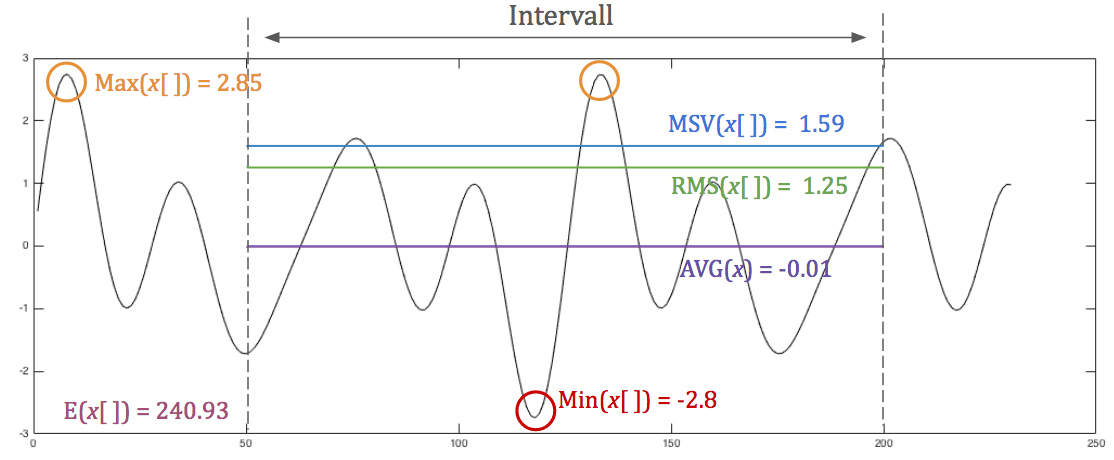
\includegraphics[width=0.7\textwidth]{bilder/sigStats02.png}
	\caption{Statistische Merkmale eines Beispielsignals über dem Intervall [50,200]}
	\label{img:sigStats}
\end{figure}

\subsection{Fehlersignale}

Angenommen, ein Signal $x[\;]$ wird übertragen, auf dem Übertragungsweg jedoch durch ein anderes Störsignal wie z.B. Rauschen $e[\;]$ überlagert. $e[\;]$ wird in diesem Zusammenhang als das \emph{Fehlersignal} bezeichnet. Das resultierende \emph{Nutzsignal} $x'[\;]$ wird nach Formel \ref{eq:sigErrorAddition} berechnet. 

\begin{equation}
x'[\;] := \quad \mathop{\forall}_{n = n_1}^{n_2} :\ x'[n] = x[n] + e[n]
\label{eq:sigErrorAddition}
\end{equation}

Eine Möglichkeit der Quantifizierung der Stärke des Rauschens im Vergleich zum Signal ist, den MSV des Eingangssignal ins Verhältnis zum MSV des Fehlersignals zu setzen. Formel \ref{eq:snrPre} gibt die Definition.

%% To do: Gute Quelle suchen!!

\begin{equation}
\text{SNR}_{rel}(x[\;],e[\;]) = \frac{MSV(x[\;])}{MSV(e[\;])}
\label{eq:snrPre}
\end{equation}

In der Praxis ist der MSV des Eingangssignals meist sehr viel höher als der des Fehlersignals. Um den Zahlenraum zu begrenzen, wird die Pseudoeinheit dB verwendet. Formel \ref{eq:snrDb} definiert den \emph{Signal/Rausch-Abstand} (\emph{SNR}, englisch Signal-to-Noise-Ratio). Ein \emph{niedriger} SNR weist auf ein \emph{starkes} Rauschen hin, und ein \emph{hoher} SNR auf ein \emph{schwaches} Rauschen. Im Zusammenhang mit der Spracherkennung ist der Signal/Rausch-Abstand von Bedeutung, da ein höheres Rauschen die Verarbeitung des Nutzsignals, der Sprache, erschwert.

\begin{equation}
\text{SNR}(x[\;],e[\;]) = 10 \cdot  \lg \Big(\frac{MSV(x[\;])}{MSV(e[\;])} \Big) \text{ dB}
\label{eq:snrDb}
\end{equation}

\subsection{Kurzzeit-Fourier-Transformation}
\label{sec:stft}

Das Signal $x[\;]$ befindet sich im \emph{Zeitbereich}, da die unabhängige Variable die Zeit definiert. Gleichung \ref{eq:complexDFTpolar} definiert die \emph{komplexe diskrete Fouriertransformation}, kurz \emph{DFT}, die das diskrete Signal $x[\;]$ aus dem Zeitbereich in den Frequenzbereich $X[\;]$ transformiert. Das Signal des Frequenzbereiches ist, ebenso wie das Signal des Zeitbereiches, $N$ punkte Lang und hat den Support $0 , \ldots , N-1$. Jedes Sample des Frequenzbereiches ist eine komplexe Zahl, deren Realteil $\Re(x[k])$ die Amplitude der entsprechenden Sinuswelle mit der Frequenz $f = k\frac{f_s}{N}$ bezeichnet und deren Imaginärteil  $\Im(x[k])$ die Amplitude der entsprechenden Kosinuswelle bezeichnet.\cite[S. 149, S. 567 - 571]{dspGuide} \cite[S. 60]{sprachverarbeitung}

\begin{equation}
\label{eq:complexDFTpolar}
\text{DFT}\{x[\;]\} = X[\;]  := \quad \mathop{\forall}_{k = 0}^{N-1} :\ X[k] =  \sum_{n = 0}^{N-1}  x[n] \cdot e^{-j 2\pi k \frac{n}{N}}
\end{equation}

Das \emph{Frequenz-Spektrum}, kurz auch nur als \emph{Spektrum} bezeichnet, wird in dieser Arbeit nach Gleichung \ref{eq:spectrum} definiert als der Absolutwert des Frequenzbereiches im Bereich $0, \ldots , N/2$.

\begin{equation}
\label{eq:spectrum}
\text{Spektrum} := \quad |X[0]| \; , \; \ldots \; , \; |X[N/2]|
\end{equation}

Abbildung \ref{img:stft01} visualisiert die Transformation in den Frequenzbereich: In der Abbildung ist oben der Zeitbereich eines 1.8 Sekunden langen Signals zu sehen. Es können klar drei nacheinander gespielte Töne erkannt werden. Der Zeitbereich lässt erkennen, zu welchen Zeitpunkten die Töne beginnen und Enden, aber nicht, welche Frequenzenkomponenten in den Tönen enthalten sind. Das heißt, es kann beispielsweise nicht erkannt werden, ob es sich um hohe oder tiefe Töne handelt. Unten ist das Spektrum abgebildet. Die x-Achse bezeichnet die Frequenz von 0 bis \SI{22050}{\hertz} und die x-Achse die Amplitude der entsprechenden Frequenz. Beide Achsen werden logarithmiert dargestellt. Das Frequenzspektrum zeigt, welche Frequenzkomponenten im dem Signal enthalten sind. So kann beispielsweise erkannt werden, dass keine Frequenzen unterhalb von \SI{1000}{\hertz} in dem Beispielsignal enthalten sind. Das Spektrum macht jedoch nicht erkennbar, zu welchen Zeitpunkten die Töne beginnen oder enden. 

\begin{figure}[h]
	\centering
	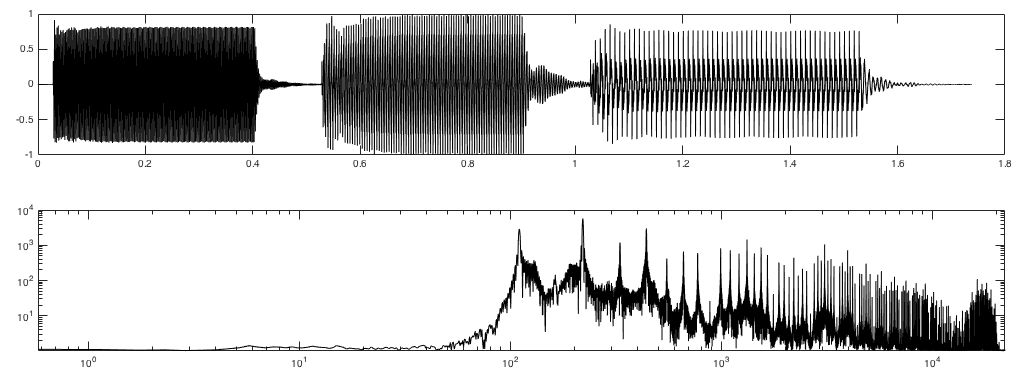
\includegraphics[width=0.8\textwidth]{bilder/stft01.png}
	\caption{Ein 1.8-Sekunden langes Signal. Oben: Der Zeitbereich mit drei klar erkennbaren Events. Unten: Das Frequenz-Spectrum des gesamten Signals mit logarithmisierten Achsen.}
	\label{img:stft01}
\end{figure}

Es ist wünschenswert, einen Kompromiss aus den Vorteilen beider Bereiche zu finden, in dem man das Spektrum kürzerer Zeitabschnitte des Signals bildet. Dazu wird der Zeitbereich $x[\;]$ in Fenster der Länge $M$ zerlegt. Die zeitliche Differenz zwischen zwei Fenstern wird als \emph{Hoptime} $R$ bezeichnet. Gleichung definiert die Bildung des \emph{Signalfensters} $x_i[\;]$. Die komplette Zerlegung eines Signals in Signalfenster wird als \emph{Windowing} bezeichnet.\cite{juliusSmith}

\begin{equation}
x_i[\;] := \quad \mathop{\forall}_{n = 0}^{M-1} :\ x_{m}[n] = x[n+i\cdot R]
\label{eq:signal-Window}
\end{equation}

Abbildung \ref{img:siganlWindows} gibt ein Beispiel für die Zerlegung eines Signals $x[\;]$ in die Signalfenster $x_0[\;] ,\ldots, x_4[\;]$. Die Samplingrate des Signals ist $f_s = 44100$, die Fensterlänge beträgt $M = 22050 / f_s = \SI{0.5}{\second}$ und die Hoptime $R = M / 2= \SI{0.25}{\second}$.

\begin{figure}[h]
	\centering
	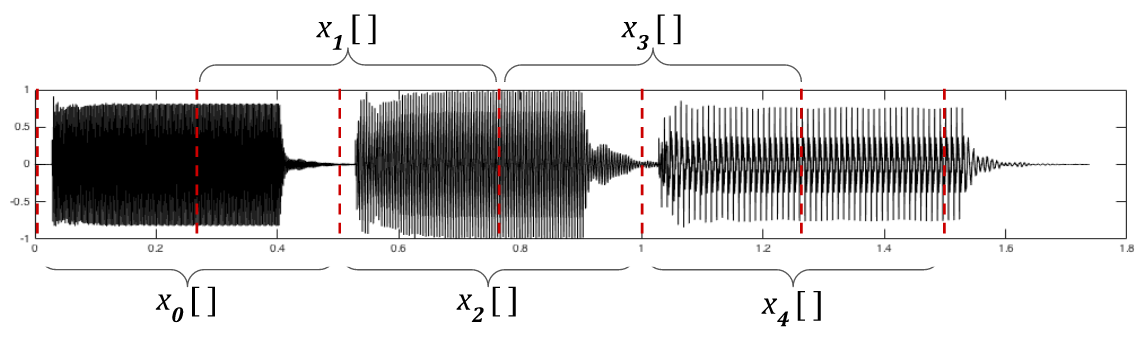
\includegraphics[width=1\textwidth]{bilder/signalWindows02.png}
	\caption{Windowing: Die Zerlegung eines Signals in kürzere Fenster.}
	\label{img:siganlWindows}
\end{figure}

Als Vorbereitungsschritt für die Transformation der Signalfenster in den Frequenzbereich wird nun jedes Fenster mit einer \emph{Fensterfunktion} (engl. \emph{window}) $w[\;]$ multipliziert.\cite[S. 69]{sprachverarbeitung} Gleichung \ref{eq:hammingWindow} definiert eine der am weitesten verbreiteten Fensterfunktionen, das \emph{Hamming-Window}. Der Paramter $M$ gibt die länge des Fensters an. Abbildung \ref{img:hamming} visualisiert das Hamming-Window. \cite[S. 286]{dspGuide}

\begin{equation}
w[\;] := \quad \mathop{\forall}_{n = 0}^{M-1} :\ w[n] = 0.54 - 0.46 \cos(\frac{2\pi n}{M} )
\label{eq:hammingWindow}
\end{equation}

\begin{figure}[h]
	\centering
	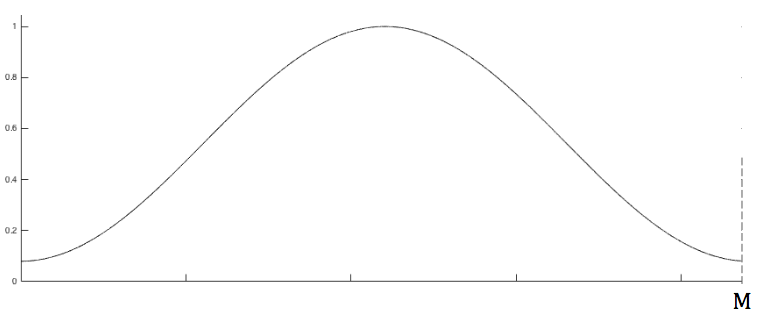
\includegraphics[width=0.4\textwidth]{bilder/hamming01.png}
	\caption{Das Hamming-Window}
	\label{img:hamming}
\end{figure}

Die Gleichung \ref{eq:stft} definiert die \emph{Kurzzeit-Fourier-Transformation} (engl. \emph{Short Time Fourier Transformation}, kurz \emph{STFT}), implementiert mit Hilfe der DFT. Dabei wird das Signalfenster $x_i[\;] = x[n+i\cdot R]$ mit der Fensterfunktion $w[\;]$ multipliziert und in das \emph{Frequenz-Fenster} $X_i[\;]$ transformiert.\cite[S. 69]{sprachverarbeitung} \cite{stft} Abbildung \ref{img:stft02} visualisiert die STFT des Beispiels aus Abbildung \ref{img:siganlWindows}.

\begin{equation}
\text{STFT}_i\{x[\;]\} = X_i[\;] := \quad \mathop{\forall}_{k = 0}^{M-1} :\ X_i[k] = \sum_{n=0}^{M-1} x[n+i\cdot R] \cdot w[n] \cdot e^{-j 2\pi k \frac{n}{N}}
\label{eq:stft}
\end{equation}

\begin{figure}[h]
	\centering
	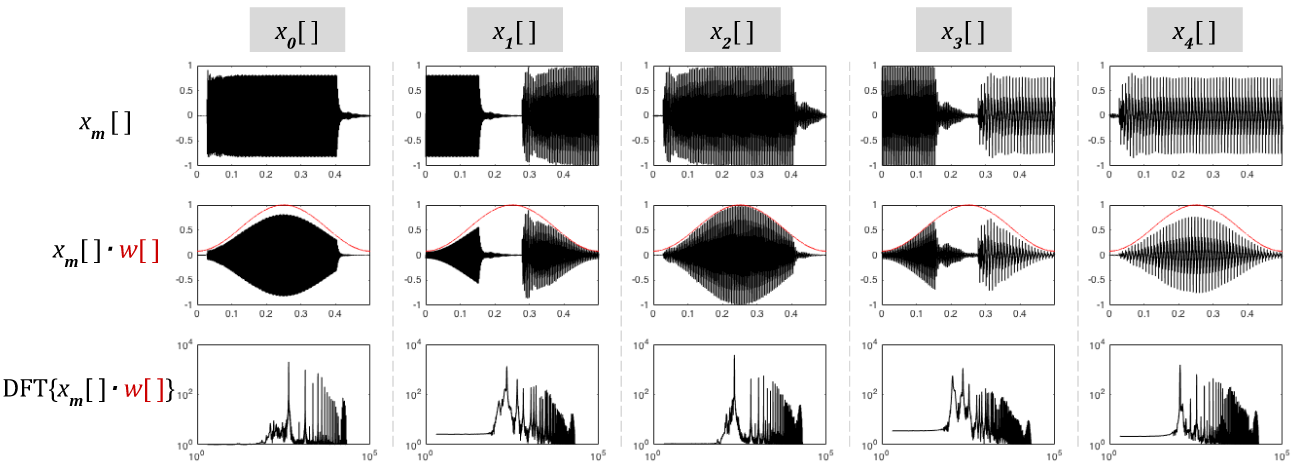
\includegraphics[width=1\textwidth]{bilder/stft03.png}
	\caption{STFT des Beispiel-Signals aus Abbildung \ref{img:siganlWindows}}
	\label{img:stft02}
\end{figure}


\subsection{Akustische Modellierung der menschlichen Stimme}
\label{sec:theVoice}

Der menschliche Sprechapparat wird in die folgenden Komponenten Unterteilt:

\begin{description}

\item[Schallproduktion: ] Die Lunge stößt Luft aus, welche die Stimmbänder passieren. Sind die Stimmbänder leicht gespannt, so wird der Luftstrom periodisch unterbrochen. Die Schwingfrequenz beträgt bei erwachsenen Männern etwa \SI{120}{\hertz} und bei Frauen \SI{220}{\hertz}. Die Frequenz kann während des Sprechens um bis zu einer Oktave variieren. Es wird so ein periodisches, akustisches Signal produziert, bezeichnet als \glqq periodische Quelle\grqq{} (engl. \glqq periodic Source\grqq). Sind die Stimmbänder stark gespannt, so entstehen Turbulenzen, die sich akustisch als ein zischendes Geräusch ohne identifizierbare Tonhöhe äußern. Dieses stimmlose Signal wird bezeichnet als \glqq Turbulenzquelle\grqq{} (engl. \glqq turbulance Source\grqq)
\item[Klangformung: ] Das Signal der Stimmlippen passiert den Rachen, Mund- und Nasenraum, welche gemeinsam als \glqq Vokaltrakt\grqq{} bezeichnet werden. Das Halszäpfchen bestimmt, ob der Luftstrom in den Mund- oder Nasenraum geleitet wird. Die Stellung der Artikulatoren, bestehend aus dem Kiefer, der Zunge usw. bestimmen die Beeinflussung des Klanges, der durch die Stimmbänder erzeugt wurde. Diese Beeinflussung wird als Filter angenähert. \cite[S. 62]{cryModel} \cite[S. 13]{sprachverarbeitung} Abbildung \ref{img:schematicVocalOrgans} visualisiert diese Komponenten.
\end{description}

\begin{figure}[h]
	\centering
	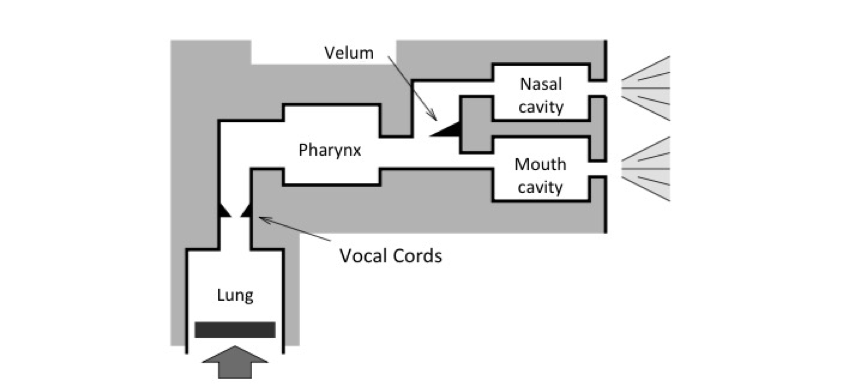
\includegraphics[width=0.7\textwidth]{bilder/SchematicVocalOrgans.png}
	\caption{Schematische Übersicht über die Organe der Spracherzeugung. Lung = Lunge, Vocal Chords = Stimmbänder, Pharynx = Rachen, Velum = Halszäpfchen, Mouth Cavity = Mundraum, Nasal Cavity = Nasenraum \cite{speechProduction}}
	\label{img:schematicVocalOrgans}
\end{figure}	

Aus Sicht der Signalverarbeitung wird die menschliche Lautproduktion durch das sogenannte \emph{Source-Filter-Modell} modelliert. Der durch die Stimmbänder erzeugte periodische Ton wird angenähert durch einen Impuls-Zug, welcher durch den Schlund als linearen Filter moduliert wird. Der stimmlose, nicht-periodische Ton wird durch weißes Rauschen angenähert. Der so erzeugte periodische oder nicht-periodische Ton wird als das Eingangssignal $u[\;]$ bezeichnet. Dieses Signal wird daraufhin an den Vokaltrakt weitergeben, welcher als lineares, zeitinvariantes Filter mit der Impulsantwort $v[\;]$ modelliert wird. Diese Impulsantwort ist abhängig von der Konfiguration der Organe des Vokaltraktes. Die Lippen werden als zweites lineares, zeitinvariantes Filter mit der Impulsantwort $r[\;]$ modelliert. $r[\;]$ wird auch als \glqq radiant Model\grqq{} bezeichnet. Das tatsächliche Sprachsignal $y[\;]$ entsteht somit durch die Faltung des Signals $u[\;]$ mit den beiden linearen, zeitinvarianten Filtern nach Gleichung \ref{eq:source-Filter-Model}. Gleichung \ref{eq:source-Filter-Model2} definiert den Frequenzbereich des Ausgangssignals $Y[\;]$ durch die Multiplikation der Frequenzbereiche der drei Komponenten. Abbildung \ref{img:source-filter-model} visualisiert diesen Prozess schematisch. \cite[S. 62 - 63]{cryModel} \cite{speechProduction}

\begin{equation}
u[\;] * v[\;] * r[\;] = y[\;] 
\label{eq:source-Filter-Model}
\end{equation}

\begin{equation}
U[\;] \cdot V[\;] \cdot R[\;] = Y[\;] 
\label{eq:source-Filter-Model2}
\end{equation}

\begin{figure}[H]
	\centering
	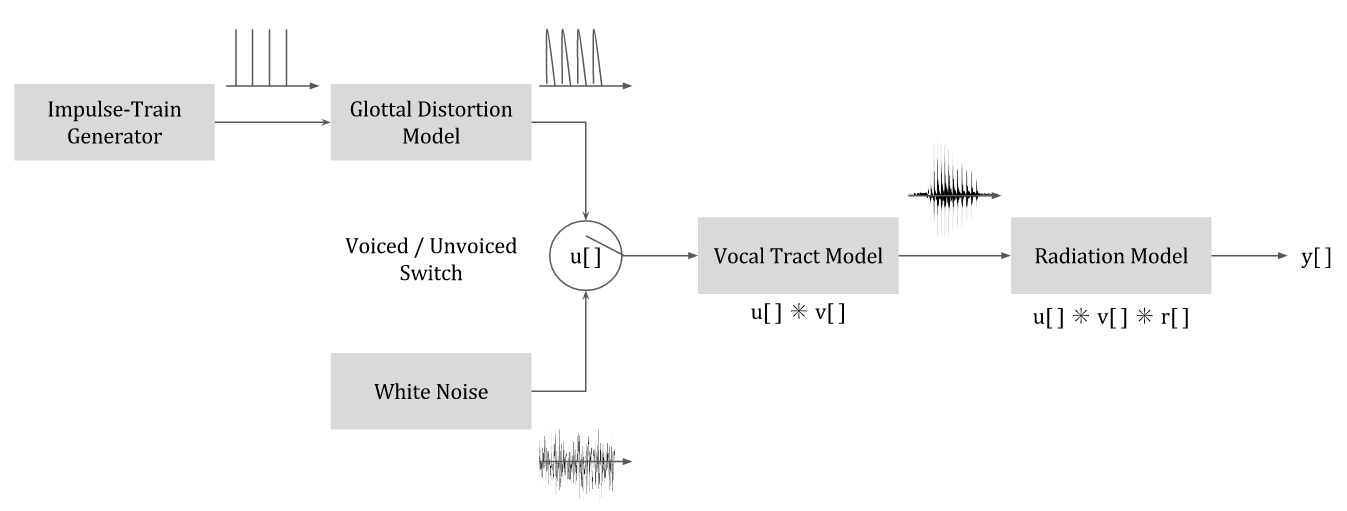
\includegraphics[width=1\textwidth]{bilder/source-filter-model.png}
	\caption{Schematische Übersicht über das Source-Filter-Model \cite[nach Source estimation, S. 17]{ricardo_ceps}}
	\label{img:source-filter-model}
\end{figure}	

Abbildung \ref{img:glottalSource} zeigt die Zeitbereiche der stimmhaften und turbulenten Quelle im Vergleich. Wie zu sehen ist, bestimmt der zeitliche Abstand zwischen den Impulsen die Grundfrequenz der Stimme. Dieses Signal $p[\;]$ wird durch den Schlund als Filter $G\{ \; \}$ gefiltert, wodurch der Zeitbereich der periodischen Quelle entsteht $G\{p[\;]\} = u_p[\;]$. Darunter ist der Zeitbereich des weißen Rauschen zu sehen. \cite[Source]{speechAcoustics}

\begin{figure}[H]
	\centering
	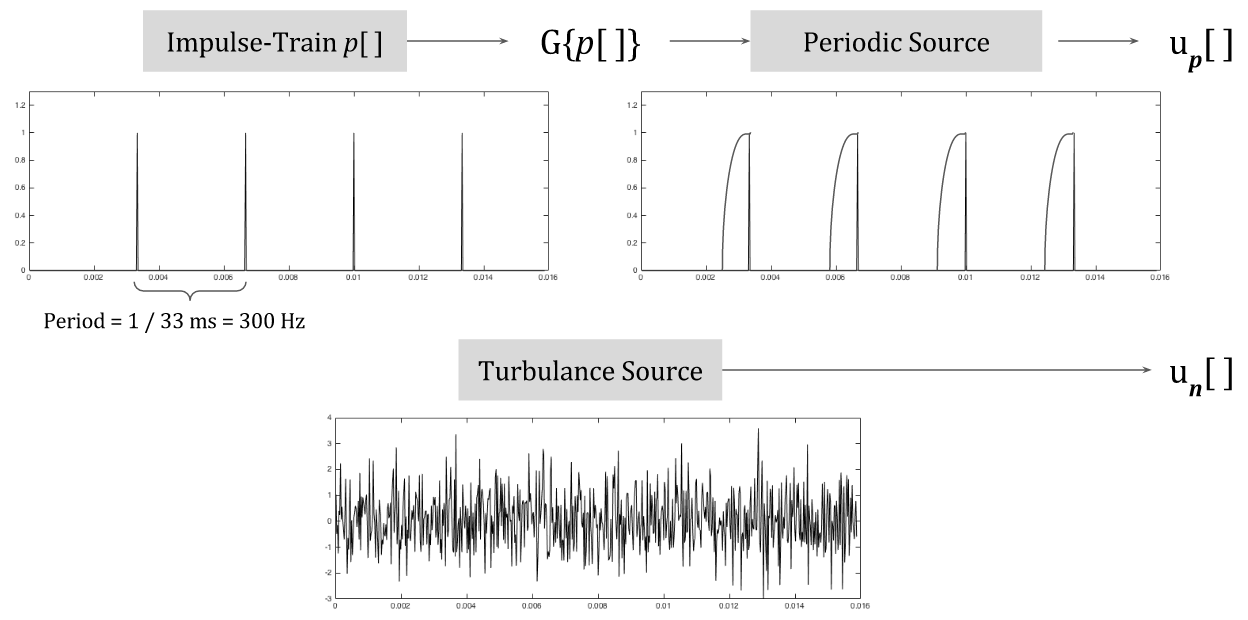
\includegraphics[width=0.8\textwidth]{bilder/glottalSource.png}
	\caption{Zeitbereiche der periodischen und der turbulenten Quelle \cite[Source]{speechAcoustics}}
	\label{img:glottalSource}
\end{figure}	

Abbildung \ref{img:sourceFilerSpectra} zeigt die Frequenzbereiche der Komponenten des Source-Filter-Modells. Die periodische Quelle ($U[\;]$ links) zeichnet sich im Frequenzbereich durch gleichmäßig verteilte Spitzen aus, die mit steigender Frequenz an Amplitude verlieren. Rechts daneben ist der Frequenzbereich des weißen Rauschen zu sehen, welcher einer Zufallsverteilung entspricht. Die Frequenzantwort des Vokaltraktes $V[\;]$ zeichnet sich durch Resonanzfrequenzen aus, von denen in diesem Beispiel vier  erkennbar sind. Die Übertragungsfunktion der Lippen $R[\;]$ wird als Hochpassfilter angenähert. Das Ausgangssignal $Y[\;] = U[\;] \cdot V[\;] \cdot R[\;]$ zeigt den Einfluss der Filter auf das jeweilige Eingangssignal.\cite[Source estimation]{ricardo_ceps}, \cite[Vocal Tract Resonance]{speechAcoustics}

\begin{figure}[H]
	\centering
	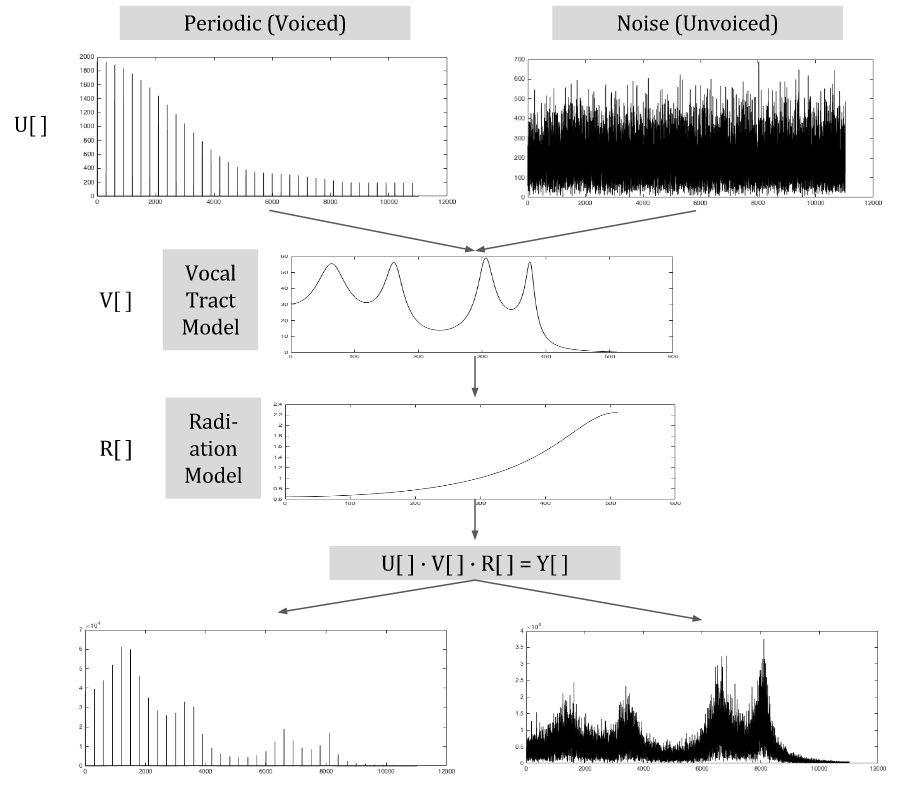
\includegraphics[width=1\textwidth]{bilder/sourceFilterSpectra.png}
	\caption{Betrachtung der Frequenzbereiche des Source-Filter-Model (nach: \cite[Source Estimation, S. 3]{ricardo_ceps})}
	\label{img:sourceFilerSpectra}
\end{figure}	

Abbildung \ref{img:pitchPeaks} zeigt schematisch das Spektrum eines stimmhaften Sprachsignals. Sowohl die Grundfrequenz als auch die harmonischen Obertonwellen sind rein visuell als \glqq viele, kurze Signalspitzen\grqq{} im Spektrum erkennbar. Der kleinste gemeinsame Teiler der Frequenzen dieser Signalspitzen entspricht der Grundfrequenz $f_0$ des Stimmsignals, in diesem Beispiel $\SI{250.7}{\hertz}$. Die Grundfrequenz ist ebenfalls an der Signalspitze mit der tiefsten Frequenz ablesbar. Die harmonischen Obertöne entsprechen der doppelten, dreifachen, \ldots Frequenz dieser Grundfrequenz, das heißt $2\cdot f_0, 3\cdot f_0, \ldots$ und werden bezeichnet mit $H_1, H_2, \ldots$. Die Grundfrequenz ist \emph{nicht zwingend} die Spitze der höchsten Amplitude. Durch den Einfluss des Vokaltraktes als Filter können harmonische Oberwellen eine höhere Amplitude als die Grundfrequenz erhalten. Auf Basis des Spektrums lässt sich somit rein visuell ein stimmhaften Signal von einem nicht stimmhaften (Rausch-)Signal unterscheiden, in dem das Spektrum nach dem Vorhandensein dieser regelmäßigen Signalspitzen überprüft wird (vergleiche mit Abbildung \ref{img:sourceFilerSpectra}).\cite[S. 52 - 53]{sprachverarbeitung}

\begin{figure}[h]
	\centering
	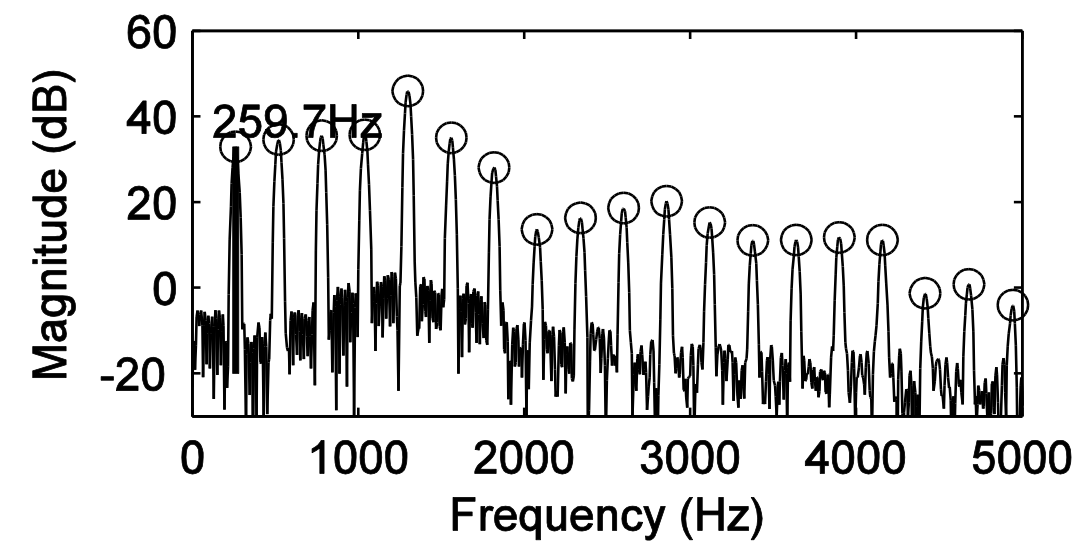
\includegraphics[width=0.5\textwidth]{bilder/pitchPeaks.png}
	\caption{Grundfrequenz und harmonische Obertöne eines periodischen Sprachsignals.}
	\label{img:pitchPeaks}
\end{figure}	

Abbildung \ref{img:formants} verdeutlicht, wie der als lineares, zeitinvariantes Filter modellierte Vokaltrakt durch Formanten bestimmt wird. Diese Formanten spielen vor allem bei der Beschreibung von Vokalen eine Rolle. Formanten sind lokale Maxima im Spektrum der Transferfunktion, die dadurch erzeugt werden, dass der Vokaltrakt Resonanzen erzeugt. Die Formanten werden von links nach rechts durchnummeriert, von $F_1 , \ldots\ , F_n$. Jeder Formant wird durch seine Mittenfrequenz, seine Bandbreite und seine Amplitude beschrieben. Das wichtigste Merkmal ist jedoch die Mittenfrequenz, da sie vom menschlichen Gehör am stärksten zur Identifikation und Unterscheidung der Vokale genutzt wird. Mit steigender Frequenz nimmt die Amplitude der Formanten ab, der dominanteste Formant ist somit immer der erste. Daher werden meist nur die ersten 2 oder 3 Formanten zur Beschreibung eines Vokals angegeben, auch, wenn theoretisch weitaus mehr vom Vokaltrakt erzeugt werden. Für verschiedene Sprachen sind allerlei Tabellen zu finden, welche die Formantenfrequenzen der Vokale auflisten.\cite[S. 19]{sprachverarbeitung}

\begin{figure}[H]
	\centering
	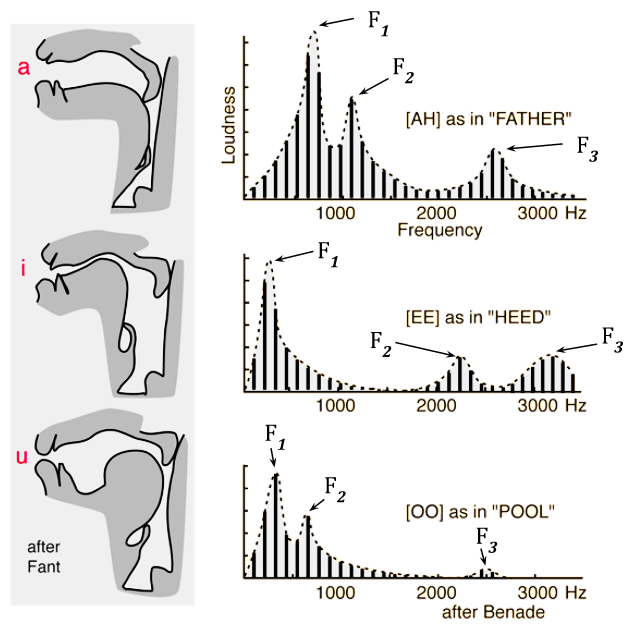
\includegraphics[width=0.7\textwidth]{bilder/formants02.png}
	\caption{Formanten im Sprach-Signal (nach: \cite{benade})}
	\label{img:formants}
\end{figure}	

Beim Sprechen befinden sich sowohl das Signal der Stimmbänder als auch das Filter des Vokaltraktes und der Lippen in ständiger Veränderung. Ein stimmhaftes Sprachsignal gilt nur über kurze Zeitbereiche weniger Millisekunden als periodisch, und selbst in diesen kurzen Zeitbereichen ist die Stimme nicht perfekt, sondern nur annähernd periodisch. Da die Informationen der Sprache vor allem im Frequenzbereich codiert sind, wird die in Kapitel \ref{sec:stft} vorgestellte Kurzzeit-Fourier-Transformation zur Analyse von Sprache eingesetzt. Die Visualisierung der STFT wird als \emph{Spektogramm} bezeichnet. Dabei werden auf der x-Achse die Zeitpunkte der Fenster und auf der y-Achse die Frequenz dargestellt. Die Frequenzfenster werden \glqq auf die Seite gelegt\grqq{}, damit ihr zeitlicher Verlauf übersichtlich betrachtet werden kann. Die Amplitude der entsprechenden Frequenzen wird farblich oder durch Helligkeiten codiert, abhängig von der konkreten Implementierung des Spektogramms. Je länger das Zeitfenster der STFT, desto höher ist die Auflösung bezüglich des Frequenzbereiches und desto niedriger die Auflösung bezüglich der Zeitbereiches. Je kürzer die Zeitfenster der STFT, desto höher ist die Auflösung bezüglich des Zeitbereiches, und desto niedriger die Auflösung des Frequenzbereiches.\cite[S. 45 - 50]{sprachverarbeitung} \cite[Acoustic Representations of Speech]{speechAcoustics}. 

Abbildung \ref{img:spectoExample} zeigt ein Beispiel für zwei Spektogramme mit unterschiedlichen Fensterlängen der STFT, angewandt auf einer 9 Sekunden langen Aufnahme eines weinenden Babys. Es ist zu erkennen, wie bei der geringeren Fensterlänge der zeitliche Verlauf besser erkennbar, jedoch die einzelnen harmonischen Obertöne weniger gut voneinander unterscheidbar sind. Bei der längeren Fensterlänge sind die Formanten leichter zu unterscheiden, der Beginn und das Ende der Lautäußerungen jedoch schwerer zu lokalisieren.

\begin{figure}[H]
	\centering
	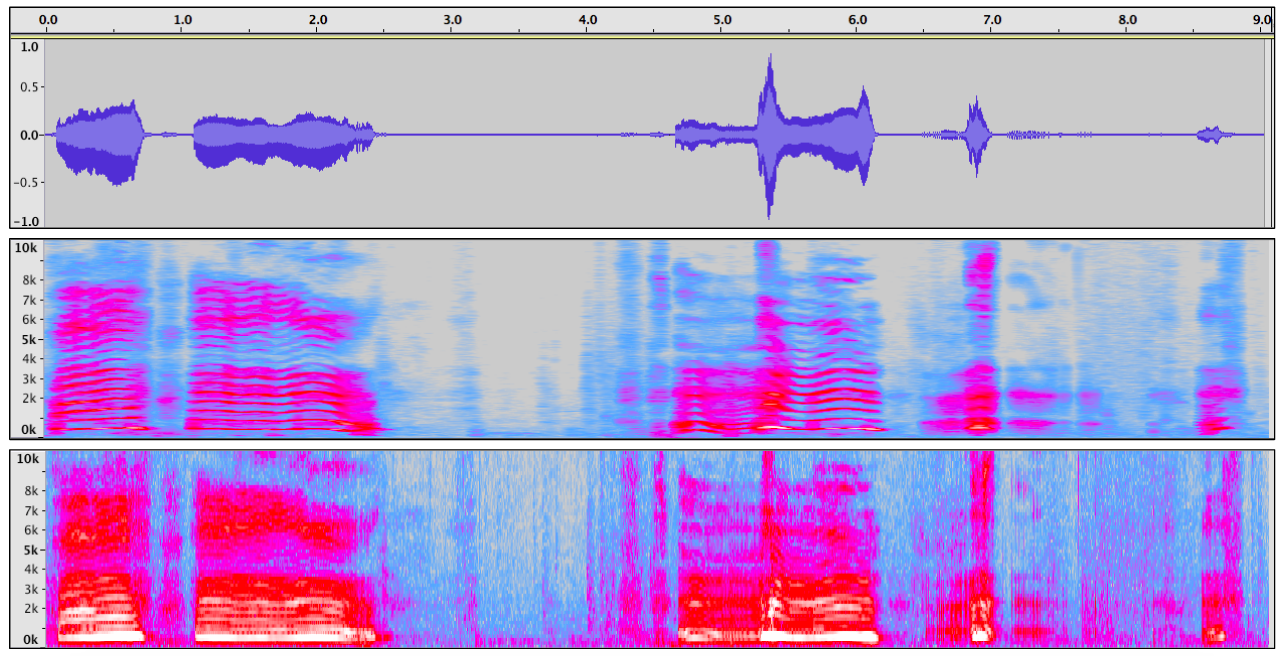
\includegraphics[width=0.8\textwidth]{bilder/spectogram03.png}
	\caption{Spektogramm einer Audioaufnahme eines Babys. Rot $\hat{=}$ hohen Amplituden, Blau $\hat{=}$ niedrigen Amplituden. Oben: Zeitbereich. Mitte: Spektogramm mit einer Fensterlänge von $\SI{185}{\milli\second}$(8192-Sample DFT). Unten: Spektogramm mit einer Fensterlänge von $\SI{5}{\milli\second}$(265-Sample DFT)}
	\label{img:spectoExample}
\end{figure}	

\section{Schreiforschung}
\label{sec:cryresearch_foundations}

Das Wissenschaftsgebiet, welches sich mit der Analyse und Interpretation von Lautäußerungen Neugeborener auseinandersetzt, wird als \glqq Schreiforschung\grqq{} bezeichnet. Die bis heute wohl prominenteste Forschungsgruppe dieses Wissenschaftsgebietes ist die in Kapitel \ref{sec:foundations_cryingMeta} erwähnte \glqq Scandinavian Cry-Group\grqq \cite{crygroup}, welche zwischen 1960 und 1990 die Laute von Babys systematisch erforscht haben. Das wichtigste Werkzeug zur Analyse der Lautäußerungen war das Spektogramm, welches damals auf analogen Technologien basierte. Das Ziel der frühen Schreiforschung war es, mit Hilfe des Spektogramms Muster zur Unterscheidung eines abnormalem Weinen von einem normalen Weinen zu finden, um beispielsweise Krankheiten erkennen zu können.\cite[S. 142]{signal} 

Teil der Scandinavian Cry-Group waren H. Golub und M. Corwin, die in der Veröffentlichung \glqq A Physioacoustic Model of the Infant Cry\grqq \cite{cryModel} ein Vokabular zur Beschreibung typischer, im Spektogramm erkennbarer Muster festgelegt haben. Da das Vokabular bis heute Einsatz findet, wird an dieser Stelle eine Übersicht über die wichtigsten Begriffe gegeben. Weiterhin werden Begriffe eingeführt, die von Zeskind et al. in \glqq Rythmic organization of the Sound of Infant Cry \grqq{} veröffentlicht wurden.\cite{rythmic}

\subsection{Phyisio-Akustische Modellierung des Weinens}
\label{sec:acousticModel}

Das Weinen von Babys lässt sich im allgemeinen als das \glqq rhythmische Wiederholen eines beim Ausatmen erzeugen Geräusches, einer kurzen Pause, einem Einatmungsgeräusch, einer zweiten Pause, und dem erneuten Beginn des Ausatmungsgeräusches\grqq beschreiben. \cite{wolff}.

Die folgenden Begriffe werden in Abbildung \ref{img:cryVocabulary} veranschaulicht.

\begin{itemize}
	\item \textbf{Expiration (Ausatmung):} Der Klang, der bei einem einzelnen, ununterbrochenen Ausatmen mit Aktivierung der Stimmbänder durch das Baby erzeugt wird. \cite{rythmic}. Der von Golub et al. \cite[S. 61]{cryModel} verwendete Begriff \textbf{Cry-Unit} wird in dieser Arbeit synonym verwendet. Umgangssprachlich ist handelt es sich um einen einzelnen, ununterbrochenen \emph{Schrei}.
	\item \textbf{Inspiration (Einatmung):} Der Klang, der beim Einatmen durch das Baby erzeugt wird.
	\item  \textbf{Burst:} Die Einheit einer Ausatmung und der darauf folgenden Einatmung. Das heisst, dass die zeitliche Dauer eines Bursts sowohl die Ausatmung, die Einatmung als auch die beiden Pausen zwischen diesen Geräuschen umfasst.\cite{rythmic}\footnote{Praktisch ergibt sich das Problem, dass vor allem bei stärkerem Hintergrundrauschen die Einatmung häufig weder hörbar noch auf dem Spektrogramm erkennbar ist. Daher wird die Zeitdauer eines Bursts von Beginn einer Ausatmung bis zum Beginn der darauf folgenden Ausatmung definiert und somit allein von den Ausatmungsgeräuschen auf die Bursts geschlossen. Implizit wird somit eine Einatmung zwischen zwei Ausatmungen angenommen.}
	\item  \textbf{Cry:} Die gesamte klangliche Antwort zu einem spezifischen Stimulus. Eine Gruppe mehrerer Cry-Units.\cite[S. 61]{cryModel} In dieser Arbeit wird ein \emph{Cry} auch als \textbf{Cry-Segment} bezeichnet, um Verwechslungen zu vermeiden.
\end{itemize}

\begin{figure}[H]
	\centering
	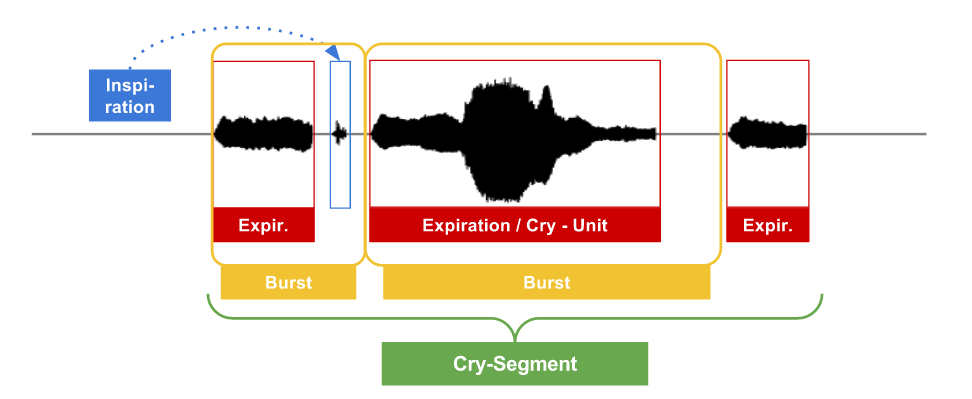
\includegraphics[width=0.8\textwidth]{bilder/cryVoc02.png}
	\caption{Veranschaulichung des Grundvokabulars}
	\label{img:cryVocabulary}
\end{figure}

Cry-Units werden von H. Golub und M. Corwin in eine der drei folgenden Kategorien eingeordnet, bezeichnet als \emph{Cry-Types}: \cite[S. 61 - 62]{cryModel}

\begin{itemize}
	\item \textbf{Phonation} beschreibt eine Cry-Unit mit einer \glqq vollen Vibration der Stimmbänder\grqq{} und einer Grundfrequenz zwischen 250 und \SI{700}{\hertz}. Entspricht umgangssprachlich einem Weinen mit einem \glqq klaren, hörbaren Ton\grqq{}.
	\item \textbf{Hyper-Phonation} beschreibt eine Cry-Unit mit einer \glqq falsetto-artigen Vibration der Stimmbänder\grqq{} mit einer Grundfrequenz zwischen 1000 und \SI{2000}{\hertz}. Entspricht umgangssprachlich einem Weinen mit einem \glqq sehr hohen, aber klar hörbaren Ton\grqq{}.
	\item \textbf{Dysphonation} beschreibt eine Cry-Unit ohne klar feststellbare Tonhöhe, produziert durch Turbulenzen an den Stimmbändern. Entspricht umgangssprachlich dem \glqq Brüllen oder Krächzen\grqq{}.
\end{itemize}

Die folgenden weiteren Eigenschaften können für einzelne Cry-Units extrahiert werden:

\begin{itemize}
	\item \textbf{Duration:} Die zeitliche Dauer der Cry-Unit.
	\item \textbf{Duration of Inspiration: }Die zeitliche Dauer der Pause zwischen zwei Cry-Units.
	\item \textbf{Grundfrequenz:} Für eine Cry-Unit kann die durchschnittliche, die höchste und die niedrigste Grundfrequenz sowie die Varianz festgestellt werden.
	\item \textbf{Frequenz der Formanten:} Wie bei der Grundfrequenz kann der Durchschnitt, das Maximum, Minimum usw. für eine Cry-Unit berechnet werden.
	\item \textbf{Ratio2: } Verhältnis zwischen den Energien der Frequenzen unterhalb von \SI{2000}{\hertz} zu den Frequenzen oberhalb von \SI{2000}{\hertz}
	\item \textbf{Cry-Mode Changes:} Häufigkeit des Wechsels des Cry-Modes innerhalb einer Cry-Unit.
	\item \textbf{Amplitude:} Die Lautstärke der Cry-Unit, gemessen in Dezibel. \cite[S. 85]{parentalPerception} \cite[S. 156]{threeCryTypes}
\end{itemize}

H. Golub und M. Corwin haben weiterhin eine Reihe von Eigenschaften vorgestellt, die das zeitliche Verhalten der Grundfrequenz und der harmonischen Obertöne innerhalb einer Cry-Unit beschreiben. \cite[S. 73]{cryModel} Einige dieser Eigenschaften werden in Abbildung \ref{img:cryMelodies} in einem schematischen Spektogramm dargestellt. Die schwarzen Linien zeigen  den Verlauf der Grundfrequenz und der Formanten.

\begin{itemize}
	\item \textbf{Pitch of Shift:} Grundfrequenz nach einem schnellen Anstieg zu Beginn der Cry-Unit
	\item \textbf{Glide:} Kurzes, starkes ansteigen der Grundfrequenz
	\item  \textbf{Glottal Roll:} Dysphonation, die häufig am Ende einer Cry-Unit nach einem Abfall der Grundfrequenz beobachtet wird.
	\item  \textbf{Vibrato:} Mehr als vier starke Schwankungen der Grundfrequenz innerhalb einer Cry-Unit.
	\item  \textbf{Melody-Type:} einer Cry-Unit. Meist: fallend, steigend/fallend, steigend, fallend/steigend, flach. 
	\item  \textbf{Continuity:} Verhältnis zwischen stimmhaften und nicht-stimmhaften Bereichen der Cry-Unit
	\item  \textbf{Double Harmonic Break:} Das Aufkommen einer zweiten Serie von harmonischen Obertönen zwischen den eigentlichen harmonischen Obertönen der Cry-Unit.
	\item  \textbf{Biphonation:} Das Aufkommen einer zweiten Grundfrequenz mit eigenen harmonischen Obertönen zusätzlich zu der eigentlichen Grundfrequenz.
	\item  \textbf{Noise Concentration:} Starke Energiespitzen zwischen 2000 und \SI{2300}{\hertz}.
	\item  \textbf{Furcation:} Plötzliches Aufteilen der Grundfrequenz und harmonischen Obertöne in mehrere, schwächere Obertöne.
\end{itemize}

\begin{figure}[H]
	\centering
	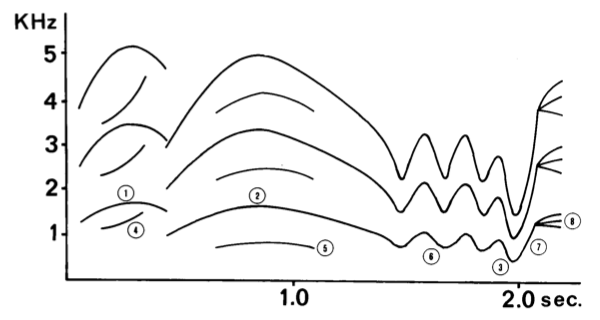
\includegraphics[width=0.7\textwidth]{bilder/melodyTypes.png}
	\caption{(1) Pitch of Shift (2) Maximale Grundfrequenz (3) Minimum der Grundfrequenz (4) Biphonation (5) Double Harmonic Break (6) Vibrato (7) Glide (8) Furcation \cite[S. 142]{signal}}
	\label{img:cryMelodies}
\end{figure}

Die folgenden Eigenschaften werden in Bezug auf das gesamte Cry-Segment, oder zumindest auf eine Menge aufeinander folgender Cry-Units berechnet:

\begin{itemize}
	\item \textbf{Cry Latence: } Zeit zwischen Stimulus, wie zum Beispiel einem Nadelstich, und der ersten Cry-Unit.
	\item \textbf{Utterances: } Anzahl der Cry-Units im Segment.
	\item \textbf{Short Utterances: } Anzahl stimmloser Cry-Units im Segment.
	\item .... und statistische Auswertungen bezüglich aller oben genannten Features, die sich auf eine Cry-Unit beziehen, wie beispielsweise der Durchschnitt aller Tonhöhen, Anzahl des Vorkommens bestimmter Melodiekonturen, Varianz der Länge der Cry-Units etc.\cite[S. 85]{parentalPerception}
\end{itemize}

Einige Krankheiten wurden in Zusammenhang mit dem vermehrten Vorkommen bestimmter Eigenschaften bei kindlichen Lautäußerungen gebracht. So wurde eine Korrelation zwischen dem Anstieg der durchschnittlichen Grundfrequenz, häufiger Biphonation und geringer Duration in Zusammenhang mit Gehirnschäden beobachtet. Tendenziell niedrige Grundfrequenzen zeigen eine Korrelation mit Trisomie 13, 18 und 21.\cite[S. 85]{parentalPerception}

\subsection{Diskussion}
\label{sec:cryDiscussion}

Bis heute bleibt die Analyse von kindlichen Lautäußerungen weitestgehend unstandartisiert: \cite[S. 142]{signal}
\begin{itemize}
	\item Es gibt keine komplette Liste, welche einen Überblick über alle berechenbaren Eigenschaften für Cry-Units oder Segmente gibt. Viele Veröffentlichungen beziehen sich auf die Eigenschaften, die von H. Golub und M. Corwin vorgestellt wurden, und erweitern diese Liste mit eigenen Vorschlägen. 
	\item Es gibt keine Einigung darüber, welche der Eigenschaften die wichtigsten sind. Beispielsweise konzentrierten sich H. Golub und M. Corwin \cite{cryModel} vermehrt auf die Erkennung von Mustern im Melodieverlauf, Zeskind et al. auf zeitliche Eigenschaften.\cite{rythmic}. Die Eigenschaft, die am häufigsten mit Schmerz, Krankheiten und sonstigen Abnormalitäten in Verbindung gebracht wird, ist eine abnormal hohe oder niedrige Tonhöhe. Bei einigen Features, die von H. Golub und M. Corwin verwendet wurden, ist nicht einmal gesichert, ob es sich nicht doch um technische Artefakte der damals verwendeten Analogtechnik handelt. \cite[S. 84 - 85]{parentalPerception}
	\item Selbst, wenn in verschiedenen Studien die selbe Eigenschaft verwendet wird, wie zum Beispiel die durchschnittliche Tonhöhe, ist nicht standardisiert, wie dieses zu berechnen ist. Mit \glqq durchschnittliche Tonhöhe des Segmentes\grqq{} kann gemeint sein: 1.) die durchschnittliche Tonhöhe, errechnet aus den durchschnittlichen Tonhöhen der der Cry-Units. 2.) Die durchschnittliche Tonhöhe aller festgestellten Tonhöhen. 3.) Die durchschnittliche Tonhöhe nur von Ausatmungslauten usw.
	\item Zusammenhänge, die zwischen bestimmten Eigenschaften des Weinens und bestimmten Krankheitsbildern festgestellt wurden, haben häufig eine hohe Spezifität, aber niedrige Sensitivität. So wurde zum Beispiel festgestellt, dass Kinder, die am plötzlichen Kindstot sterben, fast immer eine Erhöhung der Frequenz des ersten Formanten in Verbindung mit häufigen Cry-Mode-Changes zeigen. Viele Babys, die nicht am plötzlichen Kindstot sterben, zeigen jedoch die selben Merkmale.\cite[S. 85]{parentalPerception}
	\item H. Golub und M. Corwin behaupten, bereits in den achtziger Jahren ein System zur computergestützten und voll automatisierten Analyse von Cry-Segmenten implementiert zu haben. Das System nimmt 1.) eine Audioaufnahme, gespeichert auf einer Kasette an, 2.) berechnet Formanten, Grundfrequenz und Amplitude gegen die Zeit, 3.) samplt die Grundfrequenz-Kontur, 4.) berechnet insgesamt 88 akkumulierte Features für das gesamte Segment und 5.) zieht Schlussfolgerungen aus den 88 Features, wie zum Beispiel die Diagnose einer bestimmten Krankheit.\cite[S. 75 - 76]{cryModel} Abseits der kurzen Erwähnung der Existenz dieser \glqq Mutter aller automatisierten Analysesysteme für das Weinen von Babys\grqq{} konnte der Autor dieser Arbeit keine Implementierungsdetails oder sonstige genaueren Ausführungen über das System finden, welche für diese Arbeit von höchstem Interesse gewesen wären.
\end{itemize}

\section{Klassifizierung und Regression}
\label{sec:learning}

Klassifizierung und Regression sind Teilgebiete des Wissenschaftsgebietes des \emph{Überwachten Lernens}, einem Teilgebiet des Wissenschaftsgebietes des \emph{maschinellen Lernens}. Das Ziel beim Überwachten Lernen ist es, einen \emph{Prädiktor}, auch bezeichnet als\emph{Modell}, zu entwerfen, der aus den Eigenschaften einer Instanz dessen Kategorie oder Wert ableiten kann. Im Zusammenhang mit der Schreiforschung könnte eine Instanz eine Baby sein, dessen Eigenschaften 1.) die durchschnittliche Tonhöhe beim Weinen und 2.) die Augenfarbe ist. Der Prädiktor hat nun die Aufgabe, aus diesen beiden Eigenschaften eine Klasse abzuleiten, wie zum Beispiel das Geschlecht des Babys, oder einen Wert, wie beispielsweise das Alter. Das Lernen basiert dabei aus dem Generalisieren einer Liste von Beispielen, die der Algorithmus zur Verfügung gestellt bekommt. In diesem Zusammenhang wäre dies eine Liste an Babys, bei der für jede Instanz das Geschlecht oder das Alter bereits bekannt ist. Der Algorithmus versucht nun, diese Beispiele soweit zu Verallgemeinern, dass er für neue, bisher unbekannte Babys die Klasse oder den Wert korrekt voraussagen kann.\cite[S. 6 - 7]{machine_marsland}

Eine Instanz $x$ ist ein Vektor $x = ( f_1 \in F_1 , \ldots , f_n \in F_n )$. $F_i$ wird in diesem Zusammenhang als \emph{Eigenschaft}, \emph{Feature} oder \emph{Attribut} bezeichnet. In Bezug auf das eben genannte Beispiel wäre das erste Feature $F_1 = $ \emph{durschnittliche Tonhöhe} und das zweite Feature $F_2 = $ \emph{Augenfarbe}. Eine Instanz wäre in diesem Fall ein Tupel mit zwei beliebigen Werten dieser Attribute, wie zum Beispiel $x = ( \SI{300}{\hertz}, \text{blau}) )$. Features, die einen kontinuierliche Wertebereich mit einem quantitativem Charakter haben, wie zum Beispiel das Gewicht, werden als \emph{kontinuierliche} Features bezeichnet. Features, die einen diskreten Wertebereich mit einem qualitativem Charakter haben, wie zum Beispiel die Augenfarbe, werden als \emph{diskrete} Features bezeichnet.  Die Menge aller möglichen Kombination der Features $F_1 \times , \ldots , F_n$ wird als \emph{Feature-Raum} bezeichnet. Der Trainings-Datensatz $D_{trainig}$ besteht aus einer Liste an Instanzen, wobei für jede Instanz die Kategorie oder der Wert, gemeinsam Bezeichnet als \emph{Output} oder \emph{Target} $y \in Y$, bekannt ist. Ein Tupel aus einer Instanz zu einem Output wird als \emph{Example} $e =(x,y)$ bezeichnet. $Y$ bezeichnet die Menge aller möglichen Outputs des Problems. Das heißt, $D_{training} = \big( \; (x_1, y_1), \ldots , (x_N, y_N) \; \big)$. Der Prädiktor $P$ ist nun eine Funktion, die von einer Instanz auf den Output abbildet, also $P: X \mapsto Y$. Die Fehlerfunktion $E$ berechnet, wie häufig sich der Prädiktor bei der Bestimmung der Targets eines Test-Datensatzes $D_{test}$ irrt. Der Test- und der Trainings-Datensatz können die selben Instanzen, teilweise die selben oder gar keine gemeinsamen Instanzen beinhalten.\cite[S. 6 - 7, 18 - 19]{machine_marsland} \cite[S. 8 - 9]{learning_cart_dobra} 

Bei der \textbf{Klassifizierung} wird eine Target als \emph{Klasse} bezeichnet. Die Menge aller möglichen Klassen eines bestimmten Problems $Y = \{ y_1 , \ldots, y_n\}$ ist dabei diskret und hat einen \emph{qualitativen} Charakter. Das heißt, dass keine Klasse \glqq besser\grqq{} oder \glqq höher\grqq{} ist als eine andere. Ein Beispiel für ein Klassifizierungsproblem wäre die also die Ableitung des Geschlechtes für eine Instanz, also $Y = \{m, w\}$. Der Prädiktor wird in diesem Fall als Klassifikator $C$ bezeichnet.\footnote{In einigen Quellen werden die Begriffe \emph{Klassifizierung} und \emph{Klassifikation} inkonsistent verwendet. \emph{Klassifizierung} ist ein Prozess, dessen Ergebnis die \emph{Klassifikation} ist. Daher wird von einem \emph{Klassifizierungs-Algorithmus} gesprochen, da sich der Algorithmus auf den Prozess des Klassifizierens konzentriert, aber vom \emph{Klassifikationsfehler}, da der Fehler des Ergebnisses der Klassifizierung bestimmt wird. In einigen Fällen ist es unerheblich, ob das Ergebnis oder der Prozess im Fokus des Diskussionsgegenstandes steht. Dann können \emph{Klassifikation} und \emph{Klassifizierung} synonym gebraucht werden. } \cite[S. 28, 127]{statistical_learning}

Bei der \emph{Regression} ist die Menge der möglichen Targets eines bestimmten Problems \emph{kontinuierlich} und hat einen \glqq{quantitativen} Charakter. Das heißt, es kann eine interne Ordnung in der Menge der Outputs festgelegt werden. Ein Beispiel für ein Regressions-Problem wäre die also die Ableitung des Alters des Babys, also $Y = \{ 0 , \ldots , 3\}$. Der Prädiktor wird in diesem Fall auch als \emph{Regressor} $R$ bezeichnet.\cite[S. 24]{learning_cart_dobra} \cite[S. 8]{machine_marsland} \cite[S. 28]{statistical_learning}

Es gibt eine Vielzahl an Algorithmen zum Finden des Klassifikators oder Regressors. Welcher Algorithmus der \glqq beste\grqq{} ist, das heißt für einen Test-Datensatz eine möglichst hohe \emph{Genauigkeit} oder einen möglichst geringen \emph{Klassifikationsfehler} erzeugt, ist abhängig von der konkreten Problemstellung. Auf die Bestimmung der Genauigkeit wird weiter in Kapitel \ref{sec:howGoodIsMyClassifier} eingegangen. Ein Algorithmus, der in dieser Arbeit zur Klassifizierung eingesetzt wird, ist der \emph{ID3}- und der \emph{C4.5}-Algorithmus, welcher genauer in Kapitel \ref{sec:id3} beschrieben wird.

\subsection{ID3 und C4.5}
\label{sec:id3}


Der ID3-Algorithmus zählt zu den sogenannten Entscheidungsbäumen, da der durch den Algorithmus entworfene Klassifikator die Form eines Entscheidungsbaumes annimmt. Die Vorraussetzung ist, dass alle Features diskret und nicht kontinuierlich sind. Tabelle \ref{tab:id3_example} zeigt einen Beispieldatensatz zur Erläuterung des Algorithmus. Die Instanzen sind Babys, die Features die \glqq Häufigkeit des Weinens\grqq{} und die \glqq Lautstärke des Weinens\grqq{}, und die beiden Klassen \{ Ja, Nein \} geben an, ob das Kind an chronischem Schmerz leidet

\begin{table}[h]
	\centering
	\caption{Beispieldatensatz D für die Kassfikation mit ID3}
	\label{tab:id3_example}
	\begin{tabular}{cccc}
		\toprule
		$x_i$    & $f_1 \in $ Häufigkeit   & $f_2 \in $Lautstärke & $y_i$ = chron. Schmerz \\\midrule
		$x_1$  & oft                & laut          & Ja           \\
		$x_2$  & selten                & laut          & Ja           \\
		$x_3$  & normal                & leise          & Nein         \\
		$x_4$  & selten                & leise          & Nein           \\
		$x_5$  & normal                & laut         & Ja       \\
		$x_6$  & oft                & leise          & Ja       \\ \bottomrule  
	\end{tabular}
\end{table}

Abbildung \ref{img:id3tree} zeigt einen Klassifikator, den der ID-3 Algorithmus für diesen Datensatz erzeugt. Es handelt sich um einen Entscheidungsbaum. In Jedem Knoten steht ein Feature, welches einen Ast für jeden möglichen Wert dieses Features bildet. In den Blättern stehen die Klassen.\cite[S. 134]{machine_marsland}

\begin{figure}[h]
	\centering
	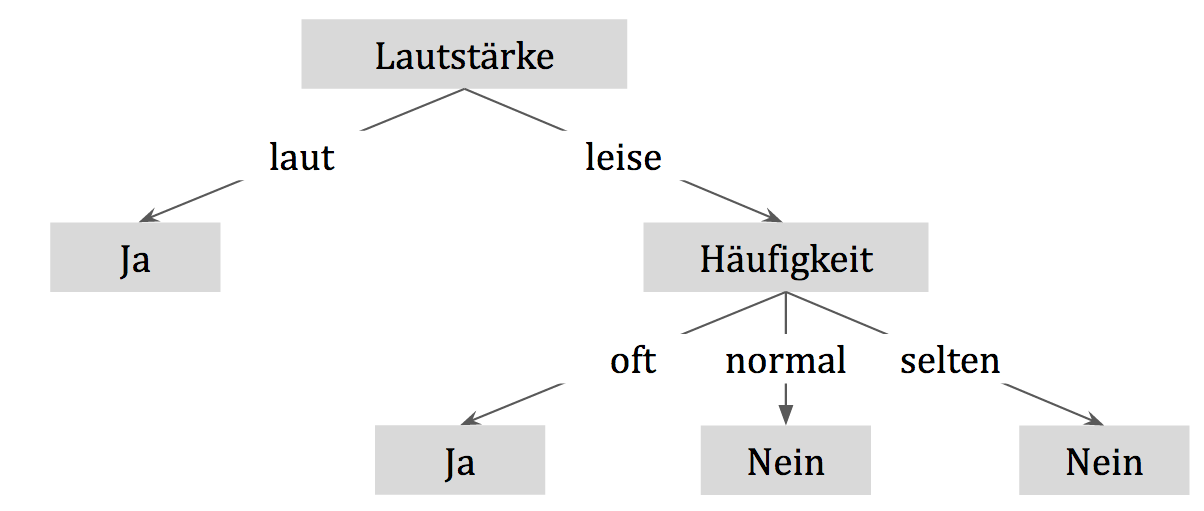
\includegraphics[width=0.6\textwidth]{bilder/id3tree02.png}
	\caption{Entscheidungsbaum, der durch den ID3-Algorithmus für den Datensatz aus Beispiel \ref{tab:id3_example} erzeugt wurde.}
	\label{img:id3tree}
\end{figure}

Der Entscheidungsbaum lässt sich in eine Reihe von \texttt{if ... then ...}-Regeln transformieren. Jeder Weg von der Wurzel bis zu einem Blatt ergibt eine Entscheidungsregel, bei der die Feauture-Werte der entsprechenden Kanten konjunktiv Verknüpft werden und die Klasse implizieren. Die Entscheidungsregeln für den Baum aus Abbildung 	\ref{img:id3tree} sind: \cite[S. 134]{machine_marsland}

\begin{itemize}
	\item \texttt{if}  \emph{Tageszeit = Tag} \texttt{then} \emph{Spaß = Ja}
	\item \texttt{if}  \emph{Tageszeit = Nacht} \texttt{and} \emph{Temperatur = warm} \texttt{then} \emph{Spaß = Ja}
	\item \ldots
\end{itemize}

Der Entscheidungsbaum wird beim ID3 Algorithmus nach folgenden Muster erstellt: Die Konstruktion wird Top-Down vollzogen, dass heisst beginnend bei der Wurzel bis zu den Blättern. In jedem Knoten wird ein Feature in alle seine möglichen Attribute aufgespalten. Um an der Wurzel zu entscheiden, welches Feature zuerst aufgespalten werden soll, wird jedes Feature einem statistischen Test unterzogen, um festzustellen, wie \glqq gut\grqq{} dieses Feauture zur Klassifikation der Trainings-Daten beiträgt. Das \glqq beste\grqq{} Attribut wird ausgewählt und als Wurzel festgelegt. Nun wird ein Kind für jeden möglichen Wert des Features gebildet. Der Datensatz des Elternknotens wird in disjunkte Teilmengen aufteilt, wobei jedes Kind die Untermenge mit denjenigen Instanzen erhält, die den jeweiligen Feature-Wert besitzen. Daraufhin beginnt für jedes Kind der Prozess des Auswählen des \glqq besten\grqq{} Attributes von vorn. Ein Kind wird dann zu einem Blatt, wenn seine Teilmenge an Daten nur noch aus Instanzen einer Klasse besteht und somit kein weiteres Aufteilen notwendig ist.\cite[S. 55]{machine_mitchell}

Zur Quantifizierung der Information wird die Entropie nach Formel \ref{eq:entropy} als Hilfsmittel definiert. $p_i$ ist die Wahrscheinlichkeit, dass in einem Datensatz $D$ ein Example mit der Klasse $i \in Y$ angetroffen wird. Die Entropie quantifiziert die \emph{Unreinheit des Datensatzes}. Ein Datensatz, dessen Instanzen alle der selben Klasse angehören, hat die Entropie $0$. Ist die \emph{Unreinheit des Datensatzes} hingegen maximal, das heißt, dass der Datensatz exakt gleich viele Instanzen jeder Klasse beinhaltet, ist die Entropie $1$. \cite[S. 135]{machine_marsland}

\begin{equation}
H(p) = -\sum_{i \in Y} p_i \cdot \log_{2} p_i
\label{eq:entropy}
\end{equation}

Es ist das Attribut in einem Knoten zu wählen, welches den höchsten \emph{Informatoinsgewinn} gewährleistet, das heißt, zu einer bestmöglichen \emph{Reinheit} in den Kindsknoten der alleinigen Unterteilung des Datensatzes auf Basis dieses Attributs führt. Der Informationsgewinn eines Features $F$ für den Datensatz $D$ wird nach Formel \ref{eq:informationGain} definiert. $f$ sind alle möglichen Werte dieses Features. $|D|$ beschreibt die Anzahl an Instanzen des Datensatzes. $D_f$ ist die Untermenge an Instanzen, die für das Feature $F$ den Wert $f$ besitzen.\cite[S. 136 - 137]{machine_marsland}

\begin{equation}
\text{Gain}(D,F) = H(D) - \sum_{f \in F} \frac{|D_f|}{|D|} H(D_f)
\label{eq:informationGain}
\end{equation}

Die Erstellung eines Entscheidungsbaumes mit Hilfe des ID3-Algorithmus wird folgendermaßen als Pseudocode definiert. Der Input des Algorithmus ist der Datensatz $D$ und der Feature-Raum $F_{all}$, der Output ist der Entscheidungsbaum.\cite[S. 139]{machine_marsland}

\vspace{5mm}

\textbf{ID3}($D,F_{all}$) \noindent\rule{0.83\linewidth}{0.3pt} \\
\begin{itemize}
\item \textbf{Wenn} alle Examples $e \in D$ das selbe Label haben:
	\begin{itemize}
	\item \textbf{return} eine Blatt mit diesem Label
	\end{itemize}
\item \textbf{Sonst: Wenn} 
	\begin{itemize}
	\item \textbf{return} ein Blatt mit dem häufigsten Label in dem Datensatz
	\end{itemize}

\item \textbf{Sonst:} 
	\begin{itemize}
	\item Wähle ein Feature $\hat{F}$ als den nächsten Knoten, dass den Informationsgewinn für den Datensatz $D$ nach Formel \ref{eq:informationGain} maximiert.
	\item Füge einen Ast für jeden möglichen Wert $f \in \hat{F}$ von dem Knoten hinzu.
	\item Für jeden Ast:
	\begin{itemize}
		\item Berechne $D_f$, in dem $\hat{F}$ von der Liste der Features entfernt wird.
		\item Rufe \textbf{ID3}($D_f, F_{all} / \hat{F}$) rekursiv auf.
	\end{itemize}
	\end{itemize}
\end{itemize}

\noindent\rule{\linewidth}{0.3pt}

\vspace{5mm}

Der ID3-Algorithmus hat folgende \textbf{Nachteile}
\begin{itemize}
\item Der Algorithmus akzeptiert keine kontinuierlichen Features.\cite[S. 72]{machine_mitchell}
\item Der Algorithmus neigt zu \emph{Overfitting}. Overfitting bedeutet, dass der Klassfikator $C$ zwar einen möglichst geringen Klassifikationsfehler in Bezug auf den Trainings-Datensatz erzeugt, es jedoch einen anderen Klassifikator $C'$ gibt, welcher für den Trainings-Datensatz einen höheren Fehler erzeugt, jedoch einen geringeren Fehler als $C$ in Bezug auf \emph{alle möglichen Instanzen dieses Typs} erzeugt. Anders formuliert bedeutet Overfitting, dass der Klassifikator den Trainings-Datensatz \glqq auswendig gelernt hat\grqq{} und nicht genügend generalisiert, um auf im Training nicht enthaltene Instanzen angewandt werden zu können. Overfitting im Zusammenhang mit dem ID-3 Algorithmus wird durch \emph{Rauschen im Trainings-Datensatz} bedingt.
\item Der Algorithmus bevorzugt greedy Attribute, die zum Zeitpunkt der Berechnung den höchsten Informationsgewinn gewährleisten. Dabei besteht die Gefahr, dass der Algorithmus in ein lokales Maximum läuft.\cite[S. 66 - 70]{machine_mitchell}
\end{itemize}

Der \emph{C4.5}-Algorithmus erweitert den \emph{ID3}, um dessen Nachteile auszumerzen, das heißt die Möglichkeit der Verwendung kontinuierlicher Attribute sowie Lösungsansätze für das Overfitting.

Bei einem kontinuierlichen Attribut wird beim \emph{C4.5}-Algorithmus im Gegensatz zu einem diskreten Attribut \emph{nicht} ein Ast für jeden möglichen Wert gebildet, sondern genau zwei Äste. Es wird also ein Grenzwert für das Feature festgelegt, bei dessen Unterschreitung der linke, und bei dessen Überschreitung der rechte Ast gewählt wird (oder, je nach Implementiert, umgedreht). Das Vorgehen zum finden eines solchen Grenzwertes ist wie folgt:

\begin{enumerate}
\item Ordne alle Examples nach ihrem jeweiligen Wertes des kontinuierlichen Feature $F_c$, für das der Grenzwert gesucht wird. 
\item Identifiziere benachbarter Examples mit unterschiedlichen Klassen. Die Feature-Werte dieser Examples sind mögliche Kandidaten für einen Grenzwert.
\item Berechne den Informationsgewinn bei Setzung des Grenzwertes auf jeden gefundenen Kandidaten. 
\item Wähle denjenigen Grenzwert, der den höchsten Informationsgewinn bringt. \cite[S. 73]{machine_mitchell}
\end{enumerate}

Abbildung \ref{img:continuos_variable} visualisiert einen Knoten mit einer kontinuierlichen Variable $F_c$, der nach einem Grenzwert in zwei Äste aufgespalten wird.


\begin{figure}[h]
	\centering
	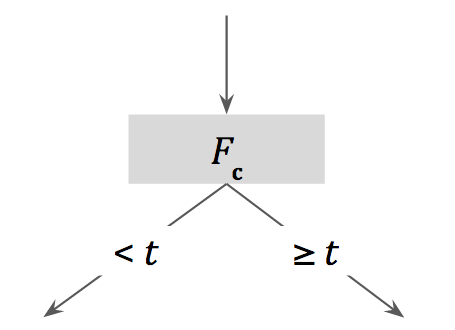
\includegraphics[width=0.3\textwidth]{bilder/continuos_variable.png}
	\caption{Aufspaltung einer kontinuierlichen Variable im Entscheidungsbaum}
	\label{img:continuos_variable}
\end{figure}


Das als Overfitting beschriebene Problem lässt sich vermeiden, in dem die Tiefe des Entscheidungsbaumes reduziert wird. Diese Begrenzung wird als \emph{Beschneiden} oder \emph{Pruning} bezeichnet. Es gibt grundlegend zwei verschiedene Ansätze:

\begin{description}
 \item[Pre-Pruning:] Ab der Überschreitung einer bestimmten Tiefe wird der Algorithmus frühzeitig gestoppt und ein Knoten, welcher die maximale Tiefe überschreitet, zwangsweise zu einem Blatt umgewandelt. \item[Post-Pruning:] Zuerst wird der komplette Entscheidungsbaum aufgebaut und Overfitting zugelassen. Im Nachhinein wird der Entscheidungsbaum in seiner Tiefe reduziert. Eines der am weitesten verbreiteten Post-Pruning-Algorithmen ist das sogenannte \emph{Reduced Error Pruning}. Dabei wird ein Knoten des Entscheidungsbaumes zu einem Blatt umgewandelt und diesem Blatt das Label zugewiesen, welches in seinem Sub-Baum am häufigsten vorkommt. Daraufhin wird der originale Entscheidungsbaum und sowie der beschnittene Entscheidungsbaum verwendet, um den Test-Datensatz zu klassifizieren. Ist der Klassifizierungsfehler des beschnittenen Baumes nicht schlechter als der des originalen Baumes, wird das Pruning übernommen. Dieses Vorgehen wird für jeden Knoten des Entscheidungsbaumes angewandt. \cite[S. 68 - 70]{machine_mitchell} 
\end{description}


\subsection{Gütemaße binärer Klassifikatoren}
\label{sec:howGoodIsMyClassifier}

Ein binärer Klassifikation ist eine, bei dem es nur zwei Klassen gibt, das heißt $|Y| = 2$. Applikationsabhängig werden die beiden Klassen beispielsweise als \emph{Positive} und \emph{Negative}, $1$ und $0$ oder \emph{True} und \emph{False} bezeichnet. Wird bei einer Klassifizierung ein tatsächliches Positive korrekt als Positive vorhergesagt wird, spricht man von einem \emph{True Positive} [TP]. Wird hingegen ein tatsächliches Positive fälschlicherweise als Negative vorhergesagt, spricht man von einem \emph{False Negative} [FN]. Bei der Klassifizierung von Negatives spricht man dementsprechend von \emph{True Negatives} [TN] und \emph{False Positives} [FP]. Die \emph{Confusion Matrix} in Abbildung \ref{img:Confusion-Matrix} gibt eine Übersicht über die vier möglichen Klassifikations-Ergebnisse. \cite[S. 213 - 214]{machine_kubat}

\begin{figure}[h]
	\centering
	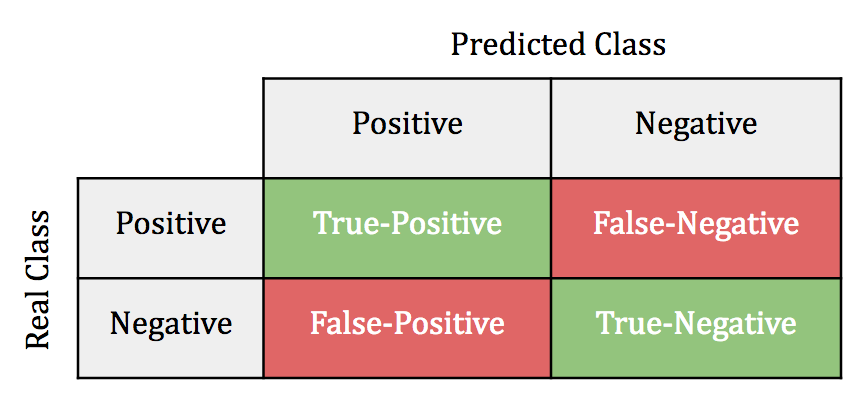
\includegraphics[width=0.4\textwidth]{bilder/Confusion-Matrix02.png}
	\caption{Confusion-Matrix (nach: \cite[S. 214]{machine_kubat})}
	\label{img:Confusion-Matrix}
\end{figure}

Die insgesamte Güte einer Klassifikation wird durch die \emph{Genauigkeit} (engl. \emph{Accuracy}) nach Formel \ref{eq:accuracy} bestimmt. Eine Genauigkeit von 100\% bedeutet, dass \emph{alle} Instanzen richtig klassifiziert wurden, eine Genauigkeit von 50\% bedeutet, dass die Hälfte aller Instanzen richtig klassifiziert wurden. Je höher die Genauigkeit, desto geringer der Klassifikationsfehler. \cite[S. 214]{machine_kubat}

\begin{equation}
\text{Accuracy} = \frac{TP+TN}{TP+TN+FN+FP}
\label{eq:accuracy}
\end{equation}

Mit Hilfe der Genauigkeit lässt sich die insgesamte Performance des Klassifikators messen. Der Wert allein gibt jedoch keinen Aufschluss darüber, ob der Klassifikator eher eine Tendenz zur falschen Klassifizierung von Positives oder Negatives hat. Bei einer Datenbank mit der selben Anzahl an Positives und Negatives kann eine Genauigkeit von 50\% beispielsweise dadurch entstehen, dass \emph{alle} Instanzen als Positives markiert werden. Das heißt, dass alle Positives richtigerweise als Positives, aber alle Negatives fälschlicherweise ebenfalls als Positives klassifiziert werden. Im Umgedrehten Fall ergibt die Klassifizierung aller Instanzen als Negatives ebenfalls eine Genauigkeit von 50\%. In einem dritten Fall irrt sich die Klassifikator gleich oft bei der Einordnung der Negatives und Positives. 

Die Maße \emph{Sensitivität} (engl. \emph{Sensitivity}) und  \emph{Spezifität} (engl. \emph{Specificity}) geben Aufschluss über die Performance des Klassifikators bei der Prädiktion der Positives und Negatives. Die Sensitivität, auch bezeichnet als \emph{True-Positive-Rate}, bemisst den Anteil tatsächlicher Positives, die auch als solche erkannt wurden, nach Formel \ref{eq:sensitivity}. Eine Sensitivität von 100\% bedeutet, dass alle in der Datenbasis enthaltenen tatsächlichen Positives auch als solche erkannt  wurden. Die Erkennungsrate der Negatives hat keinen Einfluss auf die Sensitivität. Eine hohe Sensitivität lässt sich somit \glqq einfach\grqq{} erzielen, in dem man \emph{alle} Instanzen immer als Positives klassifiziert.\cite[S. 222]{machine_kubat}

\begin{equation}
\text{Sensitivity} = \frac{TP}{TP+FN}
\label{eq:sensitivity}
\end{equation}

Die Spezifität nach Formel \ref{eq:specificity} bestimmt analog zur Sensitivität den Anteil der Negatives, die als solche klassifiziert wurden. 

\begin{equation}
\text{Specificity} = \frac{TN}{TN+FP}
\label{eq:specificity}
\end{equation}

Ein Klassifikator, der alle Instanzen als Positives markiert, hat zwar eine Sensitivität von 100\%, aber eine Spezifität von 0\%. Ergeben zwei verschiedene Klassifikationsmodelle sehr ähnliche Genauigkeiten, hilft die Bestimmung der Sensitivität und der Spezifität bei der Auswahl des für den Anwendungsfall adäquateren Klassifikators. So ist beispielsweise bei der Bestimmung von schweren Krankheiten eventuell ein Klassifikator mit höherer Sensitivtät wünschenswert, um die Wahrscheinlichkeit zu minimieren, dass die entsprechende Krankheit nicht erkannt wird. \cite{sens-and_spec}  \cite[S. 222]{machine_kubat}

